\chapter{定理证明与模型检测的结合}\label{chapt:sctl}
本章首先介绍逻辑系统\CTLP{},\CTLP{}是计算树逻辑\CTL{}的一个扩展;然后介绍针对\CTLP{}的一个证明系统\SCTL{}; 之后介绍对证明系统\SCTL{}的一个实现\sctlprov,最后介绍案例分析以及相关实验结果的对比。

\section{\CTLP{}}\label{sec:ctlp}
我们用逻辑 \CTLP{($\cal M$)} 来刻画要验证的系统 $\cal M$ 的性质,其中 $\cal M$ 通常指的是一个 Kripke 结构,其定义如下。
\begin{definition}[Kripke 结构]
	一个 Kripke 结构 $\cal M = (S, \lra, \mathcal{P})$ 包含如下三个部分:
	\begin{enumerate}
		\item $S$ 是一个有穷的状态集合;
		\item $\lra\;\subseteq S \times S$ 是一个一个二元关系 ;对于每一个状态 $s\in S$,至少存在一个 $s'\in S$ 使得 $s\lra s'$;
		\item $\mathcal{P}$ 是一个有穷的关系符号的集合;对于每个关系符号 $P\in \mathcal{P}$,都存在自然数 $n$ 使得$P\in S^n$ 。
	\end{enumerate}
\end{definition}
对于一个状态 $s\in S$,我们将 $s$ 的所有的下一个状态的集合定义为
\begin{center}
	$\nextstate{s} = \{s'\mid s\lra s'\}$。 
\end{center} 
一个路径是一个有穷或无穷的状态序列,通常形式为 $s_0,...,s_n$ 或者 $s_0,s_1,...$ ,其中,对于任意自然数$i$,如果 $s_i$ 不是该序列的最后一个元素,那么就有 $s_{i+1}\in \nextstate{s_i}$ 。

我们称 $T$ 是一棵\textit{路径树}当且仅当对于 $T$ 上的所有由 $s$ 标记的非叶子节点,该节点的所有后继节点正好由 $\nextstate{s}$ 中的所有元素一一标记。一棵路径树上的所有节点既可以是有穷个也可以是无穷个。


\paragraph{语法。}一个Kripke 结构 $\cal M$ 的性质由 \CTLP{}$(\cal M)$ 公式表示:
\begin{definition}\label{def:ctlp}
    对于一个给定的Kripke模型 $\cal M = (S, \lra, \mathcal{P})$,\CTLP{}$(\cal M)$公式的语法定义如下:
%    \begin{center}
        $$\phi \ :=
        \left\{\begin{array}{l}
        \top\ | \ \bot \ | \ P(t_1, ..., t_n)\  | \neg P(t_1, ..., t_n)\  | \ \phi  \wedge \phi \ |\ \phi \vee \phi \ | \\
        \ AX_x(\phi)(t)\ | \ EX_x(\phi)(t) \ | \ AF_x(\phi)(t) \ | \ EG_x(\phi)(t) \ |\\
        \ AR_{x,y}(\phi_1,\phi_2)(t)\ | \ EU_{x,y}(\phi_1,\phi_2)(t)
        \end{array}
        \right.$$
%    \end{center}
    其中,$x$ 与 $y$ 为变量,取值范围为 $S$,而 $t_1,...,t_n$ 既可以是代表状态的常量,也可以是取值范围为 $S$ 的变量。
\end{definition}
在定义~\ref{def:ctlp} 中,我们用模态词来绑定公式中的变量。比如,模态词 $AX$,$EX$, $AF$ 以及 $EG$ 在公式 $\phi$ 中绑定了变量 $x$;而模态词 $AR$ 和 $EU$ 则在公式 $\phi_1$ 和 $\phi_2$ 中分别绑定了变量 $x$ 和 $y$. 变量的替换则写为 $(t/x)\phi$,表示将公式 $\phi$ 中所有自由出现的变量 $x$ 都替换为 $t$。

不失一般性地来说,我们假定所有的否定符号都出现在原子命题上;而且有如下缩写:
\begin{itemize}
	\item $\phi_1\A \phi_2 \equiv \neg \phi_1 \vee \phi_2$,
	\item $EF_x(\phi)(t) \equiv EU_{z,x}(\top, \phi)(t)$,
	\item $ER_{x, y}(\phi_1,\phi_2)(t) \equiv EU_{y,z}(\phi_2,((z/x)\phi_1 \wedge
	(z/y)\phi_2))(t)\vee EG_y(\phi_2)(t)$, 其中变量 $z$ 既不在 $\phi_1$,也不在 $\phi_2$ 中出现,
	\item $AG_x(\phi)(t) \equiv \neg (EF_x(\neg \phi)(t))$,
	\item $AU_{x,y}(\phi_1,\phi_2)(t) \equiv \neg (ER_{x,y}(\neg\phi_1,\neg\phi_2)(t))$.
\end{itemize}
我们称模态词 $AF$,$EF$,$AU$,以及 $EU$ 为\textit{归纳模态词};
模态词 $AR$,$ER$,$AG$,以及 $EG$ 为\textit{余归纳模态词}。

\paragraph{语义。}相应地,对于一个给定的 Kripke 模型 $\cal M$,\CTLP{($\cal M$)}的语义定义如下:
\begin{itemize}
	\item ${\cal M}\models P(s_1,...,s_n)$:如果$\langle s_1,...,s_n\rangle\in P$,而且$P$是一个$\cal M$上的$n$元关系;
	\item ${\cal M}\models \neg P(s_1,...,s_n)$:如果$\langle s_1,...,s_n\rangle\notin P$,而且$P$是一个$\cal M$上的$n$元关系;
	\item ${\cal M}\models \top$ 永远成立;
	\item ${\cal M}\models \bot$ 永远不成立;
	\item ${\cal M}\models \phi_1\wedge\phi_2$:如果${\cal M}\models \phi_1$和 ${\cal M}\models \phi_2$同时成立;
	\item ${\cal M}\models \phi_1\vee\phi_2$:如果${\cal M}\models \phi_1$成立,或者 ${\cal M}\models \phi_2$成立;
	\item ${\cal M}\models AX_x(\phi_1)(s)$:如果对于每个状态$s'\in\textsf{Next}(s)$,都有${\cal M}\models (s'/x)\phi_1$成立;
	\item ${\cal M}\models EX_x(\phi_1)(s)$:如果存在一个状态$s'\in\textsf{Next}(s)$,使得${\cal M}\models (s'/x)\phi_1$成立;
	\item ${\cal M}\models AF_x(\phi_1)(s)$:如果存在一个有无穷个节点的树$T$,而且 $T$的根节点是$s$,那么对于$T$的任何一个非叶子节点$s'$,$s'$的子节点为\nextstate{$s'$},对于$T$的任何一个叶子节点$s'$,$\vdash (s'/x)\phi_1$成立;
	\item ${\cal M}\models EG_x(\phi_1)(s)$:如果存在$\cal M$上的一个无穷路径 $s_0,s_1,...$(其中 $s_0 = s$),那么对于任意的自然数 $i$,都有 ${\cal M}\models (s_i/x)\phi_1$成立;
	\item ${\cal M}\models AR_{x, y}(\phi_1,\phi_2)(s)$:如果存在一棵路径树 $T$,$T$ 的根节点由 $s$ 标记,对于任意节点 $s'\in T$ 都有 $\mathcal{M}\models (s'/y)\phi_2$ 成立,而且对于任意的叶子节点 $s''\in T$ 都有 $\mathcal{M}\models (s''/x)\phi_1$ 成立;
	\item ${\cal M}\models EU_{x, y}(\phi_1,\phi_2)(s)$:如果存在一个无穷路径 $s_0,s_1,...$(其中 $s_0=s$)和一个自然数 $j$,$\mathcal{M}\models(s_j/y)\phi_2$ 成立,而且对于任意的自然数 $i<j$ 都有 $\mathcal{M}\models (s_i/x)\phi_1$ 成立。
\end{itemize}


\paragraph{\CTL{} vs. \CTLP{}。}在计算树逻辑(\CTL)\cite{EmersonC82,EmersonH85} 的语法中,原子公式通常用命题符号来表示,而命题符号在计算树逻辑的语义中通常解释为一个 Kripke 结构上的状态集合。在逻辑系统\CTLP{}中,相比于计算树逻辑,我们通过引入多元谓词来增加逻辑系统中公式的表达能力。\CTLP{}相比于\CTL{}的表达能力的提升可由如下的例子表示出来:

\begin{example}\label{example:unmanned}
	本例子受多机器人路径规划系统\cite{Craig89,PartoviL14}启发。在原例子中,多机器人路径规划系统的规范可以写成 \CTL{} 公式:在一个多个区块的地图上,每从初始位置出发的机器人都能到达指定的最终位置,而且在行进的同时,每个机器人都会避免经过某些位置。
	
	在本例子中,除了\CTL{}所能表示的时序性质之外,我们考虑一种“空间”性质,即表示状态之间的关系。
	
	假定有一个无人车正在一个星球表面行驶,这个星球的表面已经被分成了有穷个小的区域。无人车一次能从一个区域行走到另一个区域,那么我们将无人车的位置看作成一个状态,无人车所有的可能的所在位置则可看作为状态空间,而且无人车从一个位置到另一个位置的移动规律则可看作成迁移关系。无人车的设计需要满足一个基本的性质,即无人车不能永远在一个很小的范围内移动。准确地说,对于给定的距离 $\sigma$,在任意状态 $s$,随着无人车的移动会到达状态 $s'$,使得 $s$ 和 $s'$ 的位置之间的距离大于 $\sigma$。该性质可以由公式 $AG_x(AF_y(D_\sigma(x,y))(x))(s_0)$ 来刻画,其中 $s_0$ 是初始状态,即无人车的降落点;原子公式 $D_\sigma(x,y)$ 则刻画了一种空间性质,即状态 $x$ 和 $y$ 的位置的距离大于 $\sigma$。
	
	\begin{figure}[h]
		\centering
		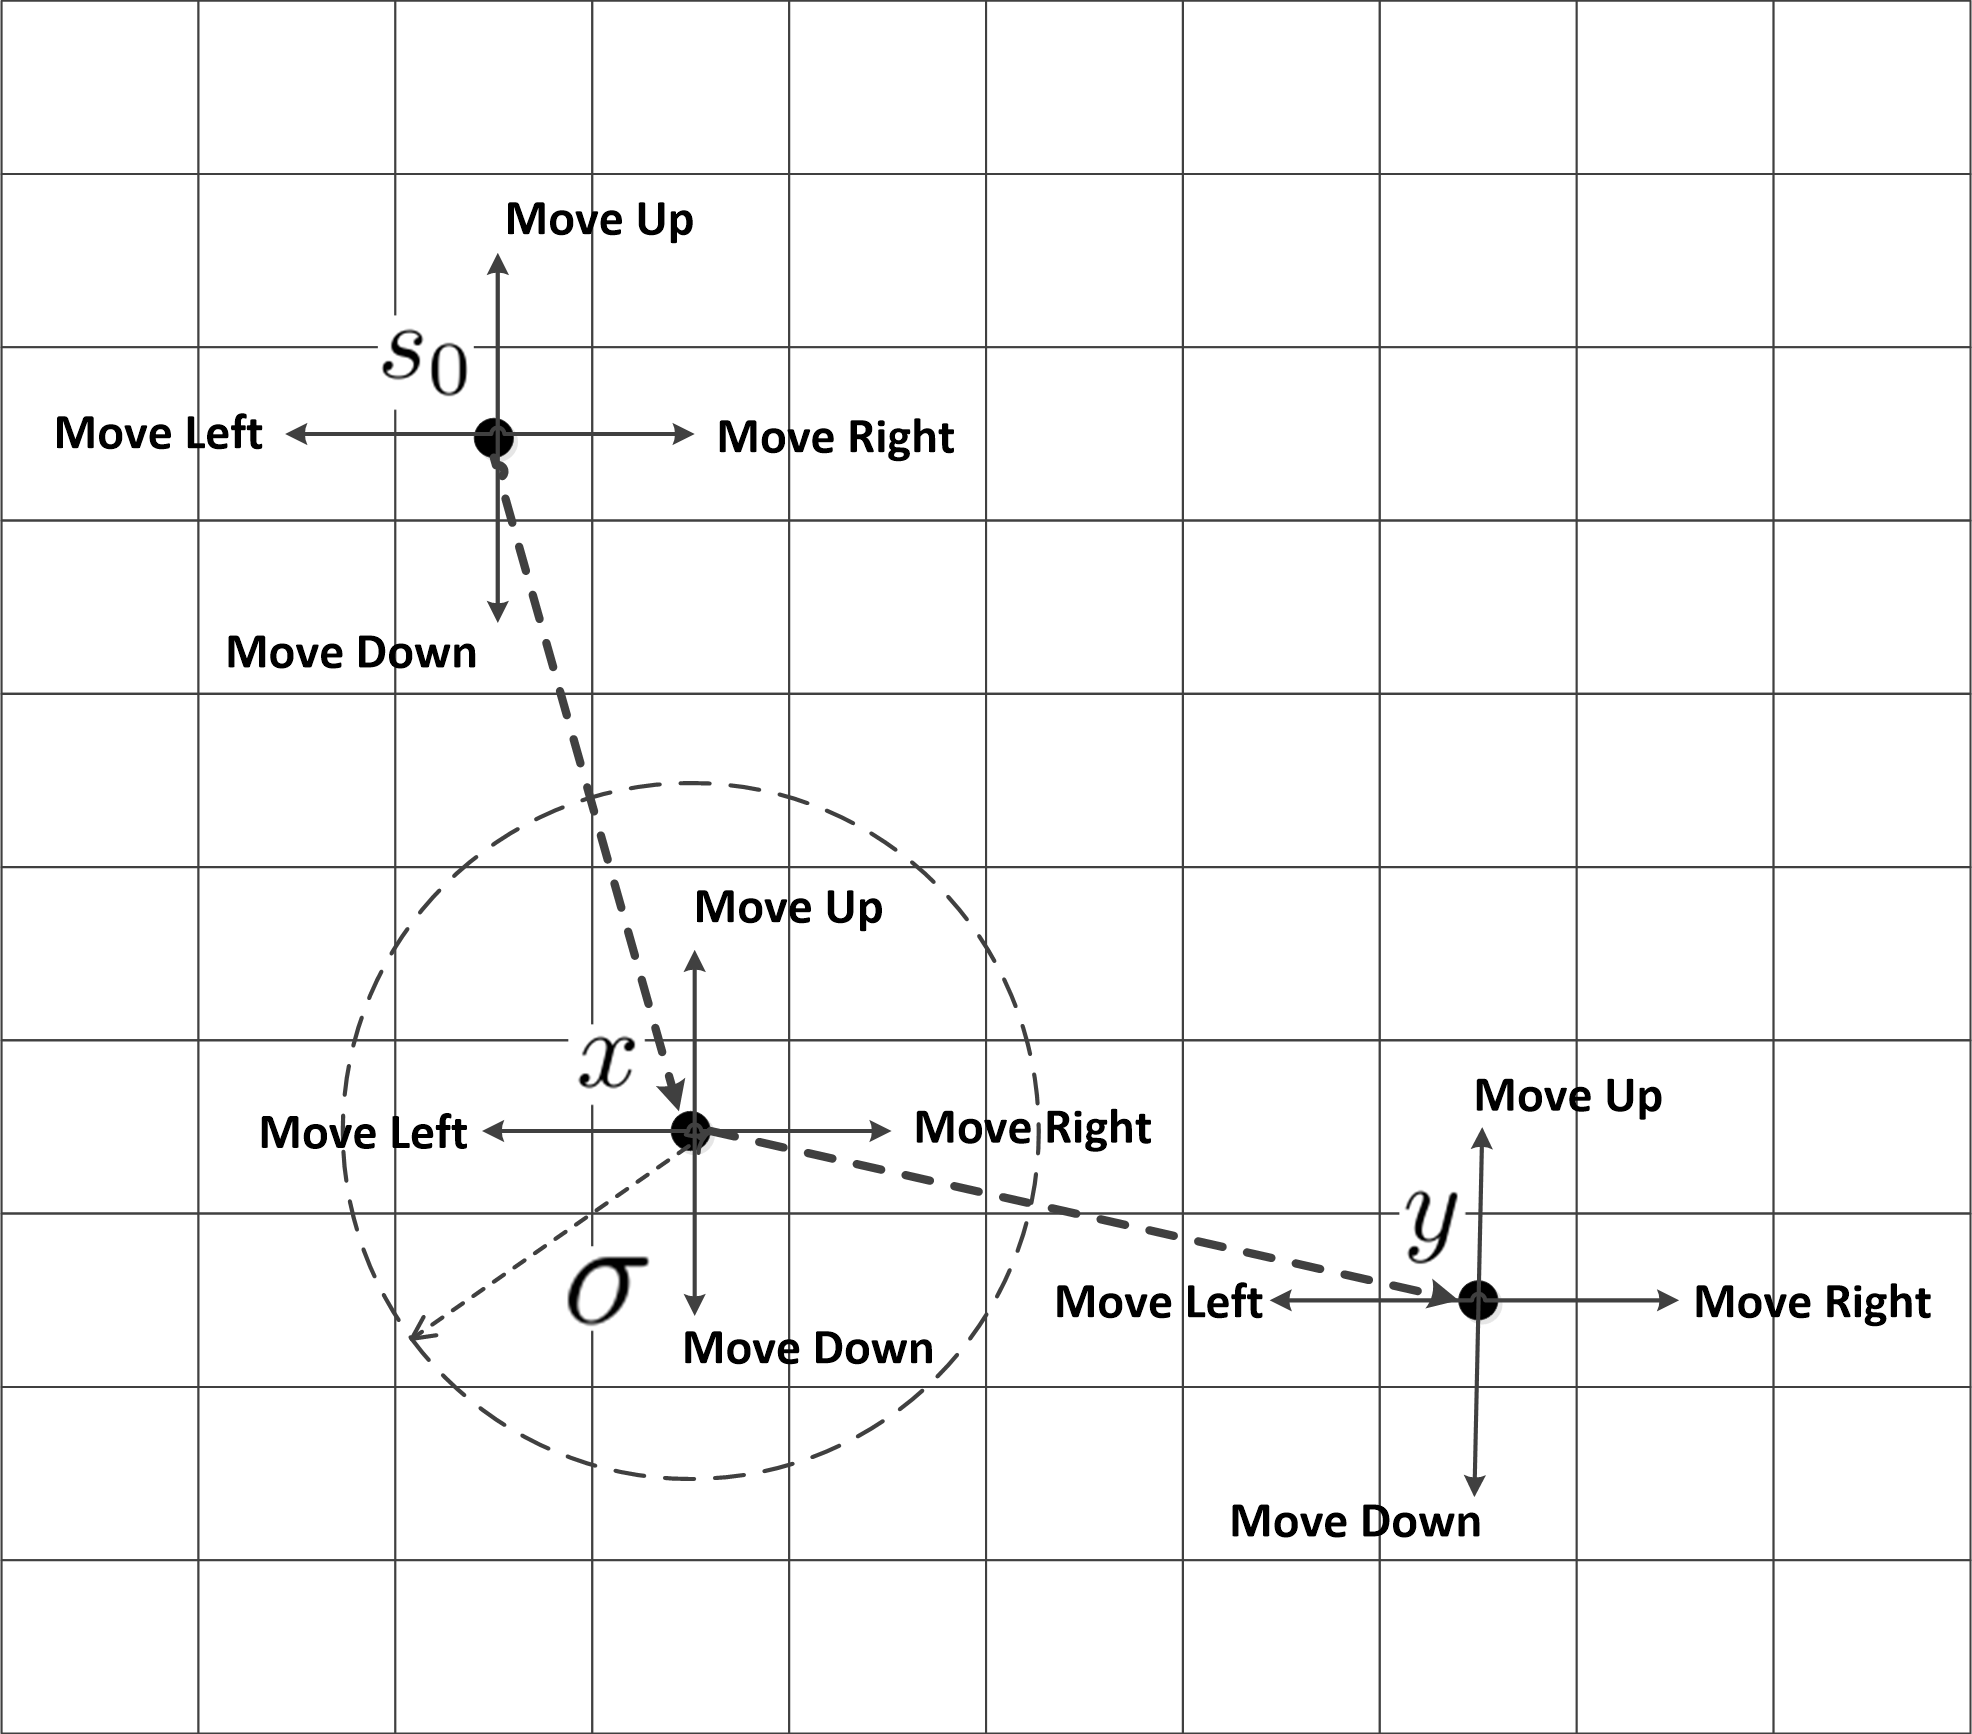
\includegraphics[width=10cm]{uv}
		\caption{无人车可能的所在位置}\label{fig:uv}
	\end{figure}
	
\end{example}

例子\ref{example:unmanned}中的性质可以很容易由 \CTLP{} 中的公式进行刻画,然而很难用传统的时序逻辑的公式进行表示。原因是在传统的时序逻辑的语法中通常没有表述一个特定的状态或者多个状态之间的关系的机制,即使在语义中,传统的时序逻辑通常只考虑当前的状态,而无法考虑多个状态之间的关系。

\section{\CTLP{}的证明系统:\SCTL{}}\label{sec:sctl}
在本节,我们针对逻辑 \CTLP$(\cal M)$ 给出一个证明系统 \sctlm{} (Sequent-calculus-like proof system for \CTLP{})。在通常意义下的证明系统中,一个公式是可证的当且仅当该公式在所有的模型中都成立,而在 \sctlm{} 中,一个公式是可证的当且仅当该公式在模型 $\cal M$ 中是可证的。

首先,让我们考虑一个\ctlpm{}公式 $AF_x(P(x))(s)$。该公式在模型 $\cal M$ 中成立当且仅当存在一个路径树 $T$,$T$ 的根节点由 $s$ 标记,而且 $T$ 上的每个叶子节点都满足 $P$。\couic{这样的路径树 $T$ 可被用来验证公式 $AF_x(P(x))(s)$ 的成立。}

然后,我们考虑一个具有嵌套模态词的 \CTLP$(\cal M)$ 公式 $AF_x(AF_y(P(x,y))(x))(s)$。如果试图说明该公式在模型 $\cal M$ 中是成立的,那么就需要找到一个路径树 $T$,使得 $T$ 的根节点由 $s$ 标记,而且对于 $T$ 中的所有叶子节点 $a$,$AF_y(P(a,y))(a)$ 是成立的。为了说明 $AF_y(P(a,y))(a)$ 是成立的,则需要又找到一棵路径树 $T'$ 使得 $T'$ 的根节点由 $a$ 标记,而且 $T'$ 上的所有叶子节点 $b$ 都满足 $P(a,b)$。我们可以用以下的两个规则来刻画当前的嵌套的路径树。
\begin{center}
	$\infer[^{\mbox{\small $\mathbf{AF}$-{$\mathsf{R_1}$}}}]{\vdash AF_x(\phi)(s)}{\vdash (s/x)\phi}$\\
	\vspace{10pt}
	$\infer[^{\mbox{\small $\mathbf{AF}$-{$\mathsf{R_2}$}}}_{\{s_1,...s_n\}=\textsf{Next}(s)}]{\vdash AF_x(\phi)(s)}
	{\vdash AF_x(\phi)(s_1) & \ldots & \vdash AF_x(\phi)(s_n)}$
\end{center}

\begin{example}\label{example:exp2}
	假设一个模型有如下图所示的迁移规则,
		\begin{center}
			\centering
			\begin{tikzpicture}
			[scale=1.5,->,>=stealth',shorten >=1pt,auto,inner sep=2pt,semithick,bend angle=20]
			\tikzstyle{every state}=[draw=none] 
			\node[state] (1) at (0,0) {$a$};
			\node[state] (2) at (1,0.3) {$b$}; 
			\node[state] (3) at (1,-0.3){$c$}; 
			\node[state] (4) at (2,0) {$d$};
			
			\draw[right] (0.1,0.05) -- (0.9,0.25);
			\draw[right] (0.1,-0.05) -- (0.9,-0.25);
			\draw[right] (1.1,0.25) -- (1.9,0.05);
			\draw[right] (1.1,-0.25) -- (1.9,-0.05);
			\draw[->] (2.1,0.1) arc (-20:-325:-0.2);
			\end{tikzpicture}
		\end{center}
		和一个原子谓词 $P=\{b, c\}$,那么公式 $AF_x(P(x))(a)$ 的一个证明如下。
		$$\infer[{\mbox{\small $\mathbf{AF}$-{$\mathsf{R_2}$}}}]{\vdash
			AF_x(P(x))(a)}{\infer[\mbox{\small $\mathbf{AF}$-{$\mathsf{R_1}$}}]{\vdash
				AF_x(P(x))(b)}{\infer[\mbox{\small atom-\textsf{R}}]{\vdash P(b)}{}} \quad\quad
			\infer[\mbox{$\mathbf{AF}$-{$\mathsf{R_1}$}}]{\vdash
				AF_x(P(x))(c)}{\infer[\mbox{\small atom-\textsf{R}}]{\vdash P(c)}{}}}$$
		在此证明树中,除了 $\mathbf{AF}$-{$\mathsf{R_1}$} 和 $\mathbf{AF}$-{$\mathsf{R_2}$},我们还应用了如下规则。 
		\begin{center}
			$\infer[^{\mbox{atom-\textsf{R}}}_{\langle s_1,...,s_n\rangle\in P}]{\vdash P(s_1,...,s_n)}{}$
		\end{center}
\end{example}


\begin{example}\label{example:exp3}
		假设另一个模型,该模型的迁移规则与例子\ref{example:exp2}中相同,除此之外还有原子谓词 $Q=\{(b,d), (c,d)\}$。
		公式 $AF_x(AF_y(Q(x, y))(x))(a)$ 的证明如下。
		
		$$\infer[{\mbox{\small $\mathbf{AF}$-{$\mathsf{R_2}$}}}]
		{\vdash AF_x(AF_y(Q(x, y))(x))(a)}
		{\infer[\mbox{$\mathbf{AF}$-{$\mathsf{R_1}$}}]
			{\vdash AF_x(AF_y(Q(x, y))(x))(b)}
			{\infer[{\mbox{\small $\mathbf{AF}$-{$\mathsf{R_2}$}}}]
				{\vdash AF_y(Q(b, y))(b)}
				{\infer[\mbox{\small $\mathbf{AF}$-{$\mathsf{R_1}$}}]
					{\vdash AF_y(Q(b, y))(d)}
					{\infer[\mbox{\small atom-\textsf{R}}]
						{Q(b,d)}
						{}
					}
				}
			}
			\quad\quad
			\infer[\mbox{$\mathbf{AF}$-{$\mathsf{R_1}$}}]
			{\vdash AF_x(AF_y(Q(x, y))(x))(b)}
			{\infer[{\mbox{\small $\mathbf{AF}$-{$\mathsf{R_2}$}}}]
				{\vdash AF_y(Q(c, y))(c)}
				{\infer[\mbox{\small $\mathbf{AF}$-{$\mathsf{R_1}$}}]
					{\vdash AF_y(Q(c, y))(d)}
					{\infer[\mbox{\small atom-\textsf{R}}]
						{Q(c,d)}
						{}
					}
				}
			}
		}$$
		
\end{example}


\couic{
	Note that \SCTL{} needs neither contraction rules nor multiplicative
$\vee$-\textsf{R} rules, because for each atomic formula $P$, either
$P$ is provable or $\neg P$ is.  Therefore the sequent $\vdash \neg P
\vee P$ is proved by proving either the sequent $\vdash \neg P$ or the
sequent $\vdash P$. 
As we have neither multiplicative $\vee$-\textsf{R} rules nor
structural rules, if we start with a sequent $\vdash \phi$ where the formula $\phi$ does not have co-inductive sub-formulae, then each
sequent in the proof has one formula on the right of $\vdash$ and none
on the left.
}
在\SCTL{}中,每个相继式都有$\Gamma\vdash\phi$形式,其中$\Gamma$是一个可能为空的\SCTL{}公式集合,$\phi$是一个\SCTL{}公式。 不同于通常的相继式演算,
%如果 $P$ 是一个原子公式,那么 $P$ 是可证的或者 $\neg P$ 是可证的。

So, as all sequents have the form $\vdash \phi$, the left rules and
the axiom rule can be dropped as well.  In other words, unlike the
usual sequent calculus and like Hilbert systems, \SCTL{} is tailored for
deduction, not for hypothetical deduction.



As the left-hand side of sequents is not used to record hypotheses, 
we will use it to record a different kind of information, that occur
in the case of co-inductive modalities, such as the modality $EG$. 

Indeed, the case of the co-inductive formula, for example $EG_x(P(x))(s)$, is
more complex than that of the inductive one, such as $AF_x(P(x))(s)$.
To justify its validity, one needs to provide an infinite sequence starting from $s$, and each state in the infinite sequence
verifies $P$. However, as the model is finite, we can always restrict to
regular sequences and use a finite representation of such sequences. This
leads us to introduce a rule, called
$\mathbf{EG}$-\textsf{merge}, that permits to prove a sequent
of the form $\vdash EG_x(P(x))(s)$, provided such a sequent already
occurs lower in the proof. To make this rule local, we re-introduce
hypotheses $\Gamma$ to record part of the history of the proof. The
sequent have therefore the form $\Gamma\vdash\phi$, with a non empty
$\Gamma$ in this particular case only, and the
$\mathbf{EG}$-\textsf{merge} rule is then just an instance of
the axiom rule, that must be re-introduced in this particular case
only.


\SCTL{$(\cal M)$} 的证明规则如图\ref{sctl_rules}所示。

\begin{figure}[h!]
	\footnotesize
	\centering
	\noindent\framebox{\parbox{.98\textwidth}{\hspace*{-0.3cm}
			$$
			\infer[^{\mbox{atom-\textsf{R}}}_{\langle s_1,...,s_n\rangle \in P}]{\vdash P(s_1,...,s_n)}{}
			\quad \quad
			\infer[^{\mbox{$\neg$-\textsf{R}}}_{\langle s_1,...,s_n\rangle \notin P}]{\vdash \neg P(s_1,...,s_n)}{}
			$$
			\smallskip
			$$
			\infer[^{\mbox{$\top$-\textsf{R}}}]{\vdash \top}{}
			\quad\quad
			\infer[^{\mbox{$\wedge$-\textsf{R}}}]{\vdash \phi_1\wedge\phi_2}{\vdash \phi_1 & \vdash \phi_2}
			\quad\quad
			\infer[^{\mbox{$\vee$-{$\mathsf{R_1}$}}}]{\vdash \phi_1\vee\phi_2}{\vdash \phi_1}
			\quad\quad
			\infer[^{\mbox{$\vee$-{$\mathsf{R_2}$}}}]{\vdash \phi_1\vee\phi_2}{\vdash \phi_2}
			$$
			\smallskip
			$$
			\infer[^{\mbox{$\mathbf{EX}$-\textsf{R}}}_{s'\in \textsf{Next}(s)}]{\vdash EX_x(\phi)(s)}{\vdash (s'/x)\phi}
			\quad\quad
			\infer[^{\mbox{$\mathbf{AX}$-\textsf{R}}}_{\{s_1,...,s_n\}=\textsf{Next}(s)}]{\vdash AX_x(\phi)(s)}{\vdash (s_1/x)\phi & \ldots & \vdash (s_n/x)\phi}
			$$
			\smallskip
			$$
			\infer[^{\mbox{$\mathbf{AF}$-{$\mathsf{R_1}$}}}]{ \vdash AF_x(\phi)(s)}{\vdash (s/x)\phi}\quad\quad
			%$$
			%$$
			\infer[^{\mbox{$\mathbf{AF}$-{$\mathsf{R_2}$}}}_{\{s_1,...,s_n\}=\textsf{Next}(s)}]{ \vdash AF_x(\phi)(s)}{\vdash AF_x(\phi)(s_1) & \ldots & \vdash AF_x(\phi)(s_n)}
			$$
			\smallskip
			$$
			\infer[^{\mbox{$\mathbf{EG}$-\textsf{R}}}_{s' \in \textsf{Next}(s)}]{\Gamma \vdash EG_x(\phi)(s)}{\vdash (s/x)\phi & \Gamma,EG_x(\phi)(s)\vdash EG_x(\phi)(s')}\quad\quad
			%$$
			%$$
			\infer[^{\mbox{$\mathbf{EG}$-\textsf{merge}}}_{EG_x(\phi)(s)\in \Gamma}]{\Gamma \vdash EG_x(\phi)(s)}{}
			$$
			\smallskip
			$$
			\infer[^{\mbox{$\mathbf{AR}$-{$\mathsf{R_1}$}}}_{\{s_1,...,s_n\}=\textsf{{Next}}(s),\Gamma' = \Gamma,AR_{x,y}(\phi_1,\phi_2)(s)}]{\Gamma \vdash AR_{x,y}(\phi_1,\phi_2)(s)}{\vdash (s/y)\phi_2 & \Gamma'\vdash AR_{x, y}(\phi_1,\phi_2)(s_1) ~...~ \Gamma'\vdash AR_{x, y}(\phi_1,\phi_2)(s_n)}
			$$
			\smallskip
			
			
			$$
			\infer[^{\mbox{$\mathbf{AR}$-{$\mathsf{R_2}$}}}]{\Gamma \vdash AR_{x,y}(\phi_1,\phi_2)(s)}{\vdash (s/x)\phi_1 & \vdash (s/y)\phi_2}
			\quad\quad
			\infer[^{\mbox{$\mathbf{AR}$-\textsf{merge}}}_{AR_{x,y}(\phi_1,\phi_2)(s)\in \Gamma}]{\Gamma \vdash AR_{x,y}(\phi_1,\phi_2)(s)}{}
			$$
			\smallskip
			$$
			\infer[^{\mbox{$\mathbf{EU}$-{$\mathsf{R_1}$}}}]{\vdash EU_{x,y}(\phi_1,\phi_2)(s)}{\vdash (s/y)\phi_2} 
			\quad\quad
			\infer[^{\mbox{$\mathbf{EU}$-{$\mathsf{R_2}$}}}_{s'\in \textsf{Next}(s)}]{\vdash EU_{x,y}(\phi_1,\phi_2)(s)}{\vdash (s/x)\phi_1 & \vdash EU_{x,y}(\phi_1,\phi_2)(s')}
			$$
			
			
	}}
	\caption{\label{sctl_rules} \sctlm{}}
\end{figure}
\paragraph{有效性与完备性。}\label{sound:complete}
%\SCTL{}证明系统的有效与完备性是基于kripke模型的有穷性。具体证明如下:
命题\ref{prop:fis}和命题\ref{prop:fit}的作用是将有穷结构转换为无穷结构,这两个命题被用来证明\SCTL{}的有效性;命题\ref{prop:ifs}和命题\ref{prop:ift}的作用是将无穷结构转换到有穷结构,这两个命题被用来证明\SCTL{}的完备性。

\begin{proposition} [有穷状态序列到无穷状态序列]\label{prop:fis}
	给定一个有穷的状态序列$s_0,...,s_n$,其中对于任意$0\le i\le n-1$都有$s_i\longrightarrow s_{i+1}$,而且存在$0\le p \le n-1$使得$s_n=s_p$。那么,一定存在一个无穷的状态序列$s_0',s_1',...$使得$s_0 = s_0'$,而且对于任意$i\ge 0$都有$s_i'\longrightarrow
	s_{i+1}'$,同时此无穷状态序列中的每个状态都在$s_0,...,s_n$中。
\end{proposition}
\begin{proof}
	本命题所述无穷序列为:$s_0,...,s_{p-1},s_p,...,s_{n-1},s_p,...$, 其中 $s_0 = s_0'$.
\end{proof}

\begin{proposition}[有穷路径树到无穷路径树]\label{prop:fit}
	设$\Phi$为一个状态集合,$T$为一个有穷的路径树,$T$的每个叶子节点都由某个状态$s$来标记,其中,$s\in \Phi$;或者存在从$T$的根结点到当前叶子节点的分支上的一个节点,使得该节点同样由$s$所标记。那么,一定存在一棵可能无穷的路径树$T'$,而且$T'$的所有叶子节点都由$\Phi$中的某个状态标记,同时用来标记$T'$节点的状态都用来标记$T$的节点。
\end{proposition}
\begin{proof}
	令$T'$的根结点为$T$的根结点,而且对于$T$的每个节点的标记$s$来说,如果$s\in\Phi$,那么$s$标记$T'$的叶子节点;否则,$s$的后继节点分别由$\mathsf{Next}(s)$中的每个元素标记。显然,标记$T'$中节点的状态都标记$T$中的节点。
\end{proof}


\begin{proposition} [无穷状态序列到有穷状态序列]\label{prop:ifs}
	给定一个无穷状态序列$s_0,s_1,...$,其中对于任意$i\ge 0$都有$s_i\longrightarrow s_{i+1}$。那么,一定存在一个有穷的状态序列$s_0',...,s_n'$,对于任意$0\le i\le n-1$,都存在一个$0\le p\le n-1$, 使得$s_n'=s_p'$,而且$s_0',...,s_n'$中的所有状态都在$s_0,s_1,...$中出现。
\end{proposition}
\begin{proof}
	由于Kripke模型的状态集是有穷的,因此在状态序列$s_0,s_1,...$一定存在$p, n\ge 0$,使得$s_p=s_n$。本命题所述有穷状态序列即为$s_0,...,s_n$。
\end{proof}

\begin{proposition}[可能无穷的路径树到有穷路径树]\label{prop:ift}
	设$\Phi$为一个状态集合;$T$为一个可能无穷的路径树,其中$T$的所有叶子节点都由$\Phi$中的某个状态所标记。那么,一定存在一个有穷的路径树$T'$,使得对于$T'$的每个叶子节点的标记$s$,$s\in\Phi$,或者存在从$T'$的根结点到该叶子节点的分支上的一个节点,该节点同样由$s$标记。
\end{proposition}
\begin{proof}
	由于Kripke模型的状态集是有穷的,因此对于$T$的每个无穷分支,都存在$0\le p<n$,使得$s_p=s_n$。将$T$的每个这样的无穷分支在$s_n$处截断,所得到的路径树即为$T'$。显然,由于$T'$具有有穷个分支,同时$T'$的每个分支都是有穷的,因此$T'$也是有穷的。
\end{proof}

\begin{theorem}[有效性]\label{thm:sound}
	设$\cal M$为一个Kripke模型,$\phi$为一个\ctlpm{}闭公式。如果相继式$\vdash\phi$具有一个证明,则$\mathcal{M}\models\phi$成立。
\end{theorem}
\begin{proof}
	假设相继式$\vdash\phi$具有证明$\pi$,以下对证明$\pi$的结构做归纳:
	\begin{itemize}
		\item 如果$\pi$的最后一条规则为\textsf{atom-R},那么$\vdash\phi$具有$\vdash P(s_1,...,s_n)$形式,因此$\mathcal{M}\models P(s_1,...,s_n)$。
		\item 如果$\pi$的最后一条规则为$\neg$-\textsf{R},那么$\vdash\phi$具有$\vdash \neg P(s_1,...,s_n)$形式,因此$\mathcal{M}\models \neg P(s_1,...,s_n)$。
		\item 如果$\pi$的最后一条规则为$\top$-\textsf{R},那么$\vdash\phi$具有$\vdash \top$形式,因此$\mathcal{M}\models \top$。
		\item 如果$\pi$的最后一条规则为$\wedge$-\textsf{R},那么$\vdash\phi$具有$\vdash \phi_1\wedge\phi_2$形式。根据归纳假设,$\mathcal{M}\models \phi_1$与$\mathcal{M}\models \phi_2$均成立,因此$\mathcal{M}\models \phi_1\wedge\phi_2$。
		\item 如果$\pi$的最后一条规则为$\vee$-\textsf{R},那么$\vdash\phi$具有$\vdash \phi_1\vee\phi_2$形式。根据归纳假设,$\mathcal{M}\models \phi_1$成立或$\mathcal{M}\models \phi_2$成立,因此$\mathcal{M}\models \phi_1\vee\phi_2$。
		
		\item 如果$\pi$的最后一条规则为$AX$-\textsf{R},那么$\vdash\phi$具有$\vdash AX_x(\phi_1)(s)$形式。根据归纳假设,对于任意$s'\in\mathsf{Next}(s)$,都有$\mathcal{M}\models (s'/x)\phi_1$成立,因此$\mathcal{M}\models AX_x(\phi_1)(s)$。
		
		\item 如果$\pi$的最后一条规则为$EX$-\textsf{R},那么$\vdash\phi$具有$\vdash EX_x(\phi_1)(s)$形式。根据归纳假设,  存在$s'\in\mathsf{Next}(s)$,使得$\mathcal{M}\models (s'/x)\phi_1$成立,因此$\mathcal{M}\models EX_x(\phi_1)(s)$。
		
		\item 如果$\pi$的最后一条规则为$\mathbf{AF}$-$\mathsf{R_1}$或$\mathbf{AF}$-$\mathsf{R_2}$,那么$\vdash\phi$具有$\vdash AF_x(\phi_1)(s)$形式。根据证明$\pi$,我们利用归纳的方式构造一棵路径树$|\pi|$。构造方式如下:
		\begin{itemize}		
			\item 如果$\pi$的最后一条规则为$\mathbf{AF}$-$\mathsf{R_1}$,而且$\rho$为$\vdash(s/x)\phi_1$的证明,则路径树$|\pi|$只包含一个节点$s$;
			
			\item 如果$\pi$的最后一条规则为$\mathbf{AF}$-$\mathsf{R_2}$,而且$\pi_1,...,\pi_n$分别为$\vdash AF_x(\phi_1)(s_1),\\...,AF_x(\phi_n)(s_n)$的证明,其中$\{s_1,...,s_n\}=\mathsf{Next}(s)$,那么令$|\pi|$等于$s(|\pi_1|,...,|\pi_n|)$。
		\end{itemize}
		%		The path-tree $|\pi|$ has root $s$, and for each leaf $s'$ of $|\pi|$, the sequent $\vdash (s'/x)\phi_1$ has a proof smaller than $\pi$. By induction hypothesis, for each leaf $s'$ of $|\pi|$, $\models (s'/x)\phi_1$. Hence $\models AF_x(\phi_1)(s)$.
		
		路径树$|\pi|$的根结点为$s$,而且对于$|\pi|$的每个叶子节点$s'$来说,$\vdash (s'/x)\phi_1$都有一个比$\pi$小的证明。根据归纳假设,对于$|\pi|$的每个叶子节点$s'$来说,都有$\mathcal{M}\models (s'/x)\phi_1$成立,因此,$\mathcal{M}\models AF_x(\phi_1)(s)$成立。
		
		
\couic{		\item If the last rule of $\pi$ is $\mathbf{EG}$-\textsf{R}, then the proved sequent has the form $\vdash EG_x(\phi_1)(s)$. We associate a finite sequence $|\pi|$ to the proof $\pi$ by induction in the following way.}
		
		\item 如果$\pi$的最后一条规则为$\mathbf{EG}$-\textsf{R},则$\vdash \phi$具有$\vdash EG_x(\phi_1)(s)$形式。根据证明$\pi$,我们归纳构造一个状态序列$|\pi|$。构造方式如下:
		\begin{itemize}
			%			\item If the proof $\pi$ ends with the $\mathbf{EG}$-merge rule, then the sequence contains a single element $s$.
			
			\item 如果$\pi$的最后一条规则为$\mathbf{EG}$-merge,那么$|\pi|$只包含一个单独的状态$s$;
			
			%			\item If the proof $\pi$ ends with the $\mathbf{EG}$-\textsf{R} rule, with subproofs $\rho$ and $\pi_1$ of the sequents $\vdash (s/x)\phi_1$ and $\Gamma, EG_x(\phi_1)(s)\vdash EG_x(\phi_1)(s')$, respectively, then $|\pi|$ is the sequence $s|\pi_1|$.
			
			\item 如果$\pi$的最后一条规则为$\mathbf{EG}$-\textsf{R},而且$\rho$和$\pi_1$分别为$\vdash(s/x)\phi_1$和$\Gamma,EG_x(\phi_1)(s)\vdash EG_x(\phi_1)(s')$的证明,其中$s'\in\mathsf{Next}(s)$,那么令$|\pi|$等于$s|\pi_1|$。
		\end{itemize}
		%		The sequent $|\pi| = s_0,s_1,...,s_n$ is such that $s_0=s$; for all $i$ between $0$ and $n-1$, $s_i\longrightarrow s_{i+1}$; for all $i$ between $0$ and $n$, the sequent $\vdash (s_i/x)\phi_1$ has a proof smaller than $\pi$; and $s_n$ is equal to $s_p$ for some $p$ between $0$ and $n-1$. By induction hypothesis, for all $i$, we have $\models (s_i/x)\phi_1$. Using Proposition \ref{prop:fis}, there exists an infinite sequence $s_0',s_1',...$ such that for all $i$, we have $s_i'\longrightarrow s_{i+1}'$, and $\models (s_i'/x)\phi_1$. Hence, $\models EG_x(\phi_1)(s)$.
		
		对于状态序列$|\pi|=s_0,...,s_n$,$s_0=s$;对于任意$0\le i\le n-1$,$s_i\longrightarrow s_{i+1}$;对于任意$0\le i\le n$,$\vdash(s_i/x)\phi_1$都有一个比$\pi$小的证明;而且存在$p<n$使得$s_n=s_p$。根据归纳假设,对于任意$i\ge 0$,都有$\mathcal{M}\models (s_i/x)\phi_1$成立。由命题\ref{prop:fis}可知,存在一个无穷的状态序列$s_0',s_1',...$,其中对于任意$i\ge 0$都有$s_i'\longrightarrow s_{i+1}'$,同时$\mathcal{M}\models (s_i'/x)\phi_1$成立。因此,$\mathcal{M}\models EG_x(\phi_1)(s)$成立。
		
\couic{		\item If the last rule of $\pi$ is $\mathbf{AR}$-$\mathsf{R_1}$ or $\mathbf{AR}$-$\mathsf{R_2}$, then the proved sequent has the form $\vdash AR_x(\phi_1,\phi_2)(s)$. We associate a finite path-tree $|\pi|$ to the proof $\pi$ by induction in the following way.}
		
		\item 如果$\pi$的最后一条规则为$\mathbf{AR}$-$\mathsf{R_1}$或$\mathbf{AR}$-$\mathsf{R_2}$,那么$\vdash \phi$具有$\vdash AR_x(\phi_1,\phi_2)(s)$形式。根据$\pi$,我们归纳构造一个有穷的路径树$|\pi|$。构造方式如下:
		\begin{itemize}
			%			\item If the proof $\pi$ ends with the $\mathbf{AR}$-$\mathsf{R_1}$ rule with subproofs $\rho_1$ and $\rho_2$ of the sequents $\vdash (s/x)\phi_1$  and $\vdash (s/x)\phi_2$, respectively, or with the
			%			$\mathbf{AR}$-merge rule, then the path-tree contains a single node $s$.
			
			\item 如果$\pi$的最后一条规则为$\mathbf{AR}$-$\mathsf{R_1}$,而且$\rho_1$和$\rho_2$分别为$\vdash (s/x)\phi_1$和$\vdash (s/x)\phi_2$的证明,那么$|\pi|$只包含一个节点$s$;
			\item 如果$\pi$的最后一条规则为$\mathbf{AR}$-merge,那么$|\pi|$只包含一个节点$s$;
			
			
			%			\item If the proof $\pi$ ends with the $\mathbf{AR}$-$\mathsf{R_2}$ rule, with subproofs $\rho, \pi_1,...,\pi_n$ of the sequents $\vdash (s/y)\phi_2$, $\Gamma, AR_{x,y}(\phi_1, \phi_2)(s) \vdash AR_{x,y}(\phi_1, \phi_2)(s_1),...,$ \\$\Gamma, AR_{x,y}(\phi_1, \phi_2)(s)\vdash AR_{x,y}(\phi_1, \phi_2)(s_n)$, respectively, then $|\pi|$ is the path-tree $s(|\pi_1|, ..., |\pi_n|)$.
			
			\item 如果$\pi$的最后一条规则为$\mathbf{AR}$-$\mathsf{R_2}$,而且$\rho, \pi_1,...,\pi_n$分别为$\vdash (s/y)\phi_2$, $\Gamma, AR_{x,y}(\phi_1, \phi_2)(s) \vdash AR_{x,y}(\phi_1, \phi_2)(s_1),...,\Gamma, AR_{x,y}(\phi_1, \phi_2)(s)\vdash AR_{x,y}(\phi_1, \phi_2)(s_n)$的证明,其中$\{s_1,...,s_n\}=\mathsf{Next}(s)$,那么令$|\pi|$等于$s(|\pi_1|, ..., |\pi_n|)$。
			
		\end{itemize}
		路径树$|\pi|$以$s$为根结点,而且对于$|\pi|$的每个节点$s'$来说,$\vdash (s'/y)\phi_2$都有一个比$\pi$小的证明;对于$|\pi|$的任意叶子节点$s'$来说,$\vdash (s'/x)\phi_1$有一个比$\pi$小的证明,或者在从$|\pi|$的根结点到当前叶子节点的分支上存在一个节点,使得$s'$标记此节点。根据归纳假设,对于$|\pi|$的任意节点$s'$,$\models (s'/y)\phi_2$成立,而且对于$|\pi|$的任意叶子节点$s'$,$\models (s'/x)\phi_1$成立,或者在从$|\pi|$的根结点到当前叶子节点的分支上存在一个节点,使得$s'$标记此节点。根据命题\ref{prop:fit},存在一个可能无穷的路径树$T'$,使得对于$T'$的每个节点$s'$,都有$\models (s'/y)\phi_2$成立,而且对于$T'$的每个叶子节点$s'$,都有$\models (s'/x)\phi_1$成立。因此,$\models AR_{x,y}(\phi_1, \phi_2)(s)$成立。
		
		%		The path-tree $|\pi|$ has root $s$, and for each node $s'$ of $|\pi|$, the sequent $\vdash (s'/y)\phi_2$ has a proof smaller than $\pi$; and for each leaf $s'$, either the sequent $\vdash (s'/x)\phi_1$ has a proof smaller than $\pi$, or $s'$ is also a label of a node on the branch from the root of $|\pi|$ to this leaf. By induction hypothesis, for each node $s'$ of this path-tree $\models (s'/y)\phi_2$ and for each leaf $s'$, either $\models (s'/x)\phi_1$ or $s'$ is also a label of a node on the branch from the root of $|\pi|$ to this leaf. Using Proposition \ref{prop:fit}, there exists a possibly
		%		infinite path-tree $T'$ such that for each node $s'$ of $T'$, $\models (s'/y)\phi_2$, and for each leaf $s'$ of $T'$, $\models (s'/x)\phi_1$. Thus, $\models AR_{x,y}(\phi_1, \phi_2)(s)$.
		
		%		\item If the last rule of $\pi$ is $\mathbf{EU}$-$\mathsf{R_1}$ or $\mathbf{EU}$-$\mathsf{R_2}$, then the proved sequent has the form $\vdash EU_{x,y}(\phi_1, \phi_2)(s)$. We associate a finite sequence $|\pi|$ to the proof $\pi$ by induction in the following way.
		
		\item 如果$\pi$的最后一条规则为$\mathbf{EU}$-$\mathsf{R_1}$或$\mathbf{EU}$-$\mathsf{R_2}$,那么$\vdash \phi$具有$\vdash EU_{x,y}(\phi_1, \phi_2)(s)$形式。根据$\pi$,我们归纳构造一个有穷状态序列$|\pi|$。构造过程如下:
		\begin{itemize}
			%			\item If the proof $\pi$ ends with the $\mathbf{EU}$-$\mathsf{R_1}$ rule with a subproof $\rho$ of the sequent $\vdash (s/y)\phi_2$, then the sequence contains a single element $s$.
			\item 如果$\pi$的最后一条规则为$\mathbf{EU}$-$\mathsf{R_1}$,那么$|\pi|$只包含一个状态$s$;
			%			\item If the proof $\pi$ ends with the $\mathbf{EU}$-$\mathsf{R_2}$ rule, with subproofs $\rho$ and $\pi_1$ of the sequents $\vdash (s/x)\phi_1$ and $\vdash EU_{x,y}(\phi_1, \phi_2)(s')$, respectively, then $|\pi|$ is the sequence $s|\pi_1|$.
			\item 如果$\pi$的最后一条规则为$\mathbf{EU}$-$\mathsf{R_2}$,而且$\rho$和$\pi_1$分别为$\vdash (s/x)\phi_1$和$\vdash EU_{x,y}(\phi_1, \phi_2)(s')$的证明,那么令$|\pi|$等于$s|\pi_1|$。
		\end{itemize}
		在状态序列$|\pi| = s_0, ..., s_n$中,$s_0=s$;对于任意$0\le i\le n-1$,$s_i \longrightarrow s_{i+1}$;对于任意$0\le i\le n-1$,$\vdash (s_i/x)\phi_1$有一个比$\pi$小的证明;而且$\vdash (s_n/y)\phi_2$有一个比$\pi$小的证明。根据归纳假设,对任意$0\le i\le n-1$,$\models (s_i/x)\phi_1$和$\models (s_n/y)\phi_2$均成立。因此,$\models EU_{x,y}(\phi_1, \phi_2)(s)$成立。
		%		The sequence $|\pi| = s_0, ..., s_n$ is such that $s_0 = s$; for each $i$ between $0$ and $n-1$, $s_i \longrightarrow s_{i+1}$; for each $i$ between $0$ and $n - 1$, the sequent $\vdash (s_i/x)\phi_1$ has a proof smaller than $\pi$; and the sequent $\vdash (s_n/y)\phi_2$ has a proof smaller than $\pi$. By induction hypothesis, for each $i$ between $0$ and $n-1$, $\models (s_i/x)\phi_1$ and $\models (s_n/y)\phi_2$. Hence, $\models EU_{x,y}(\phi_1, \phi_2)(s)$.
		%		\item The last rule cannot be a merge rule.
		\item $\pi$的最后一条规则不能为merge规则。
	\end{itemize}
\end{proof}

\begin{theorem}[完备性]\label{thm:complete}
	设$\phi$是一个\ctlpm{}闭公式。如果$\mathcal{M}\models\phi$,则$\vdash\phi$在\SCTL$(\cal M)$中是可证的。
\end{theorem}
\begin{proof}
	对$\phi$的结构作归纳:
	%	By induction over the size of $\phi$.
	\begin{itemize}
		%		\item If $\phi = P(s_1,...,s_n)$, then as $\models P(s_1,...,s_n)$, the sequent $\vdash P(s_1,...,s_n)$ is provable with the rule \textsf{atom-R}.
		
		\item 如果$\phi = P(s_1,...,s_n)$,那么由$\mathcal{M}\models P(s_1,...,s_n)$可知,$\vdash P(s_1,...,s_n)$是可证的。
		
		%		\item If $\phi = \neg P(s_1,...,s_n)$, then as $\models \neg P(s_1,...,s_n)$, the sequent $\vdash \neg P(s_1,...,s_n)$ is provable with the rule $\neg$-\textsf{R}.
		
		\item 如果$\phi = \neg P(s_1,...,s_n)$,那么由$\mathcal{M}\models \neg P(s_1,...,s_n)$可知,$\vdash \neg P(s_1,...,s_n)$是可证的。
		
		%		\item If $\phi = \top$, then $\vdash \top$ is provable with the rule $\top$-\textsf{R}.
		
		\item 如果$\phi = \top$,那么显然$\vdash \top$是可证的。
		
		%		\item If $\phi = \bot$, then it is not the case that $\models \bot$.
		\item 如果$\phi = \bot$,那么显然$\vdash \bot$是不可证的。
		
		%		\item If $\phi = \phi_1\wedge\phi_2$, then as $\models \phi_1\wedge\phi_2$, $\models \phi_1$ and $\models \phi_2$. By induction hypothesis, the sequents $\vdash \phi_1$ and $\vdash \phi_2$ are provable. Thus the sequent $\vdash \phi_1\wedge\phi_2$ is provable with the $\wedge$-\textsf{R} rule.
		
		\item 如果$\phi = \phi_1\wedge\phi_2$,那么由于$\mathcal{M}\models \phi_1\wedge\phi_2$,因此$\mathcal{M}\models \phi_1$和$\mathcal{M}\models \phi_2$均成立。根据归纳假设,$\vdash \phi_1$和$\vdash \phi_2$均可证。因此,$\vdash \phi_1\wedge\phi_2$是可证的。
		
		%		\item If $\phi = \phi_1\vee\phi_2$, as $\models \phi_1\vee\phi_2$, $\models \phi_1$ or $\models \phi_2$. By induction hypothesis, the sequent $\vdash \phi_1$ or $\vdash \phi_2$ is provable and the sequent $\vdash \phi_1\vee\phi_2$ is provable with the $\vee$-$\mathsf{R_1}$ or $\vee$-$\mathsf{R_2}$ rule, respectively.
		
		\item 如果$\phi = \phi_1\vee\phi_2$,那么由于$\mathcal{M}\models \phi_1\vee\phi_2$,因此$\mathcal{M}\models \phi_1$或 $\mathcal{M}\models \phi_2$成立。根据归纳假设,$\vdash \phi_1$或$\vdash \phi_2$是可证的。因此,$\vdash \phi_1\vee\phi_2$是可证的。
		
		%		\item If $\phi = AX_x(\phi_1)(s)$, as $\models AX_x(\phi_1)(s)$, for each state $s'$ in $\textsf{Next}(s)$, we have $\models (s'/x)\phi_1$. By induction hypothesis, for each $s'$ in $\textsf{Next}(s)$, the sequent $\vdash (s'/x)\phi_1$ is provable. Using these proofs and the $\mathbf{AX}$-\textsf{R} rule, we build a proof of the sequent $\vdash AX_x(\phi_1)(s)$.
		
		\item 如果$\phi = AX_x(\phi_1)(s)$,那么由于$\mathcal{M}\models AX_x(\phi_1)(s)$,因此对于任意$s'\in \mathsf{Next}(s)$,都有$\mathcal{M}\models (s'/x)\phi_1$成立。根据归纳假设,对于任意$s'\in \mathsf{Next}(s)$,$\vdash (s'/x)\phi_1$都是可证的。因此,$\vdash AX_x(\phi_1)(s)$是可证的。
		
		%		\item If $\phi = EX_x(\phi_1)(s)$, as $\models EX_x(\phi_1)(s)$, there exists a state $s'$ in $\textsf{Next}(s)$ such that $\models (s'/x)\phi_1$. By induction hypothesis, the sequent $\vdash (s'/x)\phi_1$ is
		%		provable. With this proof and the $\mathbf{EX}$-\textsf{R} rule, we build a proof of the sequent $\vdash EX_x(\phi_1)(s)$.
		
		\item 如果$\phi = EX_x(\phi_1)(s)$,那么由于$\mathcal{M}\models EX_x(\phi_1)(s)$,因此存在$s'\in \mathsf{Next}(s)$使得$\mathcal{M}\models (s'/x)\phi_1$成立。根据归纳假设,$\vdash (s'/x)\phi_1$是可证的,因此$\vdash EX_x(\phi_1)(s)$是可证的。
		%		\item If $\phi = AF_x(\phi_1)(s)$, as $\models AF_x(\phi_1)(s)$, there exists a finite path-tree $T$ such that $T$ has root $s$, for each internal node $s'$, the children of this node are labeled by the elements of $\textsf{Next}(s')$, and for each leaf $s'$, $\models (s'/x)\phi_1$. By induction hypothesis, for every leaf $s'$, the sequent $\vdash (s'/x)\phi_1$ is provable. Then, to each subtree $T'$ of $T$, we associate a proof $|T'|$ of the sequent $\vdash AF_x(\phi_1)(s')$ where $s'$ is the root of $T'$, by induction, as follows.
		\item 如果$\phi = AF_x(\phi_1)(s)$,那么由于$\mathcal{M}\models AF_x(\phi_1)(s)$,因此存在一棵有穷的路径树$T$,并且$T$以$s$为根结点;对于$T$的每个非叶子节点$s'$,$s'$的后继节点分别由$\mathsf{Next}(s)$中的元素所标记;对于$T$的每个叶子节点$s'$,都有$\mathcal{M}\models (s'/x)\phi_1$成立。根据归纳假设,$\vdash (s'/x)\phi_1$是可证的。然后,对于$T$的每个以子树$T'$(设$T'$的根结点为$s'$),我们归纳构造$\vdash AF_x(\phi_1)(s')$的一个证明$|T'|$。构造过程如下:
		\begin{itemize}
			%			\item If $T'$ contains a single node $s'$, then the proof $|T|$ is built with the $\mathbf{AF}$-$\mathsf{R_1}$ rule from the proof of $\vdash (a/x)\phi_1$ given by the induction hypothesis.
			
			\item 如果$T'$只包含一个节点$s'$,那么$|T'|$的最后一条规则为$\mathbf{AF}$-$\mathsf{R_1}$,同时$|T'|$中包含$\vdash (s'/x)\phi_1$的证明;
			%			\item If $T' = s'(T_1, ..., T_n)$, then the proof $|T|$ is built with the $\mathbf{AF}$-$\mathsf{R_2}$ rule from the proofs $|T_1|, ..., |T_n|$ of the sequents $\vdash AF_x(\phi_1)(s_1), ..., \vdash AF_x(\phi_1)(s_n)$, respectively, where $s_1, ..., s_n$ are the elements of $\textsf{Next}(s')$.
			
			\item 如果$T' = s'(T_1, ..., T_n)$,那么$|T'|$的最后一条规则为$\mathbf{AF}$-$\mathsf{R_2}$,同时$|T_1'|,...,|T_n'|$分别为$\vdash AF_x(\phi_1)(s_1), ..., \vdash AF_x(\phi_1)(s_n)$的证明,其中\\$\{s_1, ..., s_n\}=$ $\mathsf{Next}(s)$。 
		\end{itemize}
		
		%		This way, the proof $|T|$ is a proof of the sequent $\vdash AF_x(\phi_1)(s)$.
		因此,$|T|$是$\vdash AF_x(\phi_1)(s)$的一个证明。
		
		\item 如果$\phi = EG_x(\phi_1)(s)$,那么由于$\mathcal{M}\models EG_x(\phi_1)(s)$,因此存在一个状态序列$s_0,...,s_n$使得$s_0=s$,而且对于任意$0\le i\le n$都有$\mathcal{M}\models (s_i/x)\phi_1$成立。根据归纳假设,$\vdash (s_i/x)\phi_1$是可证的。根据命题\ref{prop:ifs},存在一个有穷的状态序列$T=s_0,...,s_n$使得对任意$0\le i\le n-1$,$s_i \longrightarrow s_{i+1}$,同时$\vdash (s_i/x)\phi_1$是可证的,而且存在$p<n$使得$s_n=s_p$。
		对于$T$的每个后缀$s_i,...,s_n$,我们归纳构造$|s_i,...,s_n|$为$EG_x(\phi_1)(s_0),\ldots, EG_x(\phi_1)(s_{i-1}) \vdash EG_x(\phi_1)(s_i)$的证明。构造方式如下:
			
		\begin{itemize}

				\item $|s_n|$的最后一条规则为$\mathbf{EG}$-merge;
				
				\item 如果$i \le n-1$,根据归纳假设,由于$\vdash (s_i/x)\phi_1$是可证的,而且$|s_{i+1}, ..., s_n|$是$EG_x(\phi_1)(s_0), ..., EG_x(\phi_1)(s_i) \vdash EG_x(\phi_1)(s_{i+1})$的一个证明。因此,$|s_i, ..., s_n|$是$EG_x(\phi_1)(s_0),\ldots, EG_x(\phi_1)(s_{i-1}) \vdash EG_x(\phi_1)(s_i)$的一个证明,而且最后一条规则为$\mathbf{EG}$-\textsf{R}。
				
		\end{itemize}
			
		因此,$|s_0,...,s_n|$是$\vdash EG_x(\phi_1)(s)$的一个证明。

		\item 如果$\phi = AR_{x,y}(\phi_1, \phi_2)(s)$,那么由于$\mathcal{M}\models AR_{x,y}(\phi_1, \phi_2)(s)$,因此存在一棵以$s$为根节点的可能无穷的路径树,对于该路径树的每个节点$s'$,都有$\mathcal{M}\models (s'/x)\phi_2$;对于该路径树的每个叶子节点$s'$,都有$\mathcal{M}\models (s'/x)\phi_1$。根据归纳假设,对于该路径树的每个节点$s'$,$\vdash (s'/y)\phi_2$是可证的,而且对于该路径树的每个叶子节点$s'$,$\vdash (s'/y)\phi_1$是可证的。由命题\ref{prop:ift}可知,存在一棵有穷的路径树$T$,对于该路径树的每个节点$s'$,$\vdash (s'/y)\phi_2$是可证的;对于该路径树的每个叶子节点$s'$,$\vdash (s'/y)\phi_1$是可证的,或者$s'$为从$T$的根节点到该叶子节点分支上的节点。然后,对于$T$的每个子树$T'$,我们归纳构造$AR_{x,y}(\phi_1, \phi_2)(s_1), ..., AR_{x,y}(\phi_1,
		\phi_2)(s_m) \vdash AR_{x,y}(\phi_1, \phi_2)(s')$的一个证明$|T'|$,其中$s'$为$T'$的根节点,而且$s_1,...,s_m$为从$T$的根节点到$T'$的根节点的分支。构造方式如下:
		\begin{itemize}

			\item 如果$T'$只包含一个单独的节点$s'$,同时$\vdash (s'/x)\phi_1$是可证的,那么根据归纳假设,$\vdash (s'/x)\phi_1$和$\vdash (s'/y)\phi_2$皆可证,而且$|T'|$的最后一条规则为$\mathbf{AR}$-$\mathsf{R_1}$;

			\item 如果$T'$只包含一个单独的节点,同时$s'$包含在$s_1,...,s_m$中,那么$|T'|$的最后一条规则为$\mathbf{AR}$-merge;
			
			\item 如果$T' = s'(T_1, ..., T_n)$,那么根据归纳假设,$|T_1|,...,|T_n|$分别为
			\begin{center}
				$AR_{x,y}(\phi_1,\phi_2)(s_1),...,AR_{x,y}(\phi_1,\phi_2)(s_m)$, $AR_{x,y}(\phi_1,\phi_2)(s')\vdash AR_{x, y}(\phi_1,\phi_2)(s_1')$\\
				...\\
				$AR_{x,y}(\phi_1,\phi_2)(s_1),...,AR_{x,y}(\phi_1,\phi_2)(s_m)$, $AR_{x,y}(\phi_1,\phi_2)(s')\vdash AR_{x, y}(\phi_1,\phi_2)(s_n')$
			\end{center}
			的证明,同时$|T'|$的最后一条规则为$\mathbf{AR}$-$\mathsf{R_2}$,其中$s_1',...,s_n'=\mathsf{Next}(s')$。
			
		\end{itemize}
		
		因此,$|T|$是$\vdash AR_{x,y}(\phi_1,\phi_2)(s)$的一个证明。
		

		\item 如果$\phi = EU_{x,y}(\phi_1, \phi_2)(s)$,那么由于$\mathcal{M}\models EU_{x,y}(\phi_1, \phi_2)(s)$,因此存在一个有穷的状态序列$T = s_0, ..., s_n$使得$\mathcal{M}\models (s_n/y)\phi_2$成立,而且对于任意$0\le i\le n-1$,$\mathcal{M}\models (s_i/x)\phi_1$成立。根据归纳假设,$\vdash (s_n/y)\phi_2$是可证的,而且对于任意$0\le i\le n-1$,$\vdash (s_i/x)\phi_1$是可证的。然后,对于$T$的每个后缀$s_i,...,s_n$,我们归纳构造$|s_i, ..., s_n|$为$\vdash EU_{x,y}(\phi_1, \phi_2)(s_i)$的证明。构造方式如下:
		
		\begin{itemize}

			\item $|s_n|$的最后一条规则为$\mathbf{EU}$-$\mathsf{R_1}$;

			
			\item 如果$i\le n-1$,那么根据归纳假设,由于$|s_{i+1},...,s_n|$是$\vdash EU_{x,y}(\phi_1,\phi_2)(s_{i+1})$的证明,而且$\vdash (s_i/x)\phi_1$是可证的,因此,$|s_i,...,s_n|$是$\vdash EU_{x,y}(\phi_1, \phi_2)(s_i)$的证明。
		\end{itemize}

		
		因此,$|s_0,...,s_n|$是$\vdash EU_{x,y}(\phi_1,\phi_2)(s)$的一个证明。
	\end{itemize}
	
\end{proof}


\section{\SCTL{}的工具实现:\sctlprov{}}\label{sec:sctlprov}
本节介绍\SCTL{}的一个实现---\sctlprov{}(图\ref{workflow})以及该工具与其他模型检测工具的对比。
\sctlprov{}的工作方式如下:首先,\sctlprov{}读入一个输入文件,并将该输入文件解析到一个Kripke模型以及若干个\SCTL{}公式;然后,对于每个公式,\sctlprov{}搜索该公式的证明,如果该公式可证,则并输出该证明(或者只输出True),如果该公式不可正,则输出该公式的非的证明(或者只输出False)。


\begin{figure}[h]
	\centering
	\makebox[0.60\textwidth][c]{%
		\tiny
		\begin{tikzpicture}[
		outpt/.style={->,blue!80!black,very thick},
		outpt1/.style={->,red!80!black,very thick},
		>=stealth,
		every node/.append style={align=center}]
		
		\node [inputfile] (input) at (0,0) {
			\begin{tabular}{@{}c}
			\textsf{Input}\\\textsf{file}
			\end{tabular}};
		
		\node (preproc) at (1.5,0) {\textsf{Interpret}};
		
		\draw[outpt](input)--(preproc);
		
		\node (proofsearch) at (3.0,0) {
			\begin{tabular}{@{}l}
			\textsf{Proof}\\
			\textsf{search}
			\end{tabular}};
		
		\draw[outpt](preproc)--(proofsearch);
		
		\node [inputfile] (prooftree) at (7,1) {
			\begin{tabular}{@{}c}
			\textsf{Certificate} \\\textsf{or True}
			\end{tabular}};
		
		%\node (result) at (9, 0) {Provable/Unprovable};
		\node [inputfile] (result) at (7, -1) {
			\begin{tabular}{@{}c}
			\textsf{Counterexample} \\\textsf{or False}
			\end{tabular}};
		
		\node (sctlprov) at (2,0.5) {\sctl{}};
		\node (output) at (4.0,0.1) {\textsf{output}};
		\node (provable) at (5.3, 1.1) {\textsf{provable}};
		\node (unprovable) at (5.3,-1.15) {\textsf{unprovable}};
		
		%\node (output) at (6, 0.2) {output?};
		%\node (yes) at (6.85, 0.5) {yes};
		
		
		\begin{pgfonlayer}{background}
		\path (preproc.west |- sctlprov.north)+(-0.2,0.1) node (a) {};
		\path (proofsearch.east |- proofsearch.south)+(+0.2,-0.2) node (c) {};
		\path[fill=yellow!30,rounded corners, draw=black!50]
		(a) rectangle (c);
		\end{pgfonlayer}
		
		\begin{pgfonlayer}{background}
		\path (preproc.west |- preproc.north)+(-0.1,0.1) node (a) {};
		\path (preproc.east |- preproc.south)+(+0.1,-0.1) node (c) {};
		\path[fill=green!30,rounded corners, draw=black!50]
		(a) rectangle (c);
		\end{pgfonlayer}
		
		\begin{pgfonlayer}{background}
		\path (proofsearch.west |- proofsearch.north)+(-0.1,0.1) node (a) {};
		\path (proofsearch.east |- proofsearch.south)+(+0.1,-0.1) node (c) {};
		\path[fill=green!30,rounded corners, draw=black!50]
		(a) rectangle (c);
		\end{pgfonlayer}
		
		%\draw[blue!80!black,very thick, dashed](6.6, 0)--(6.6, 1);
		%\draw[blue!80!black,very thick](6.6, 1)--(prooftree);
		\draw[-,very thick, blue!80!black](3.55, 0)--(4.5, 0);
		\draw[-,very thick, blue!80!black](4.5, 0)--(4.5, 1);
		\draw[-,very thick, blue!80!black](4.5, 0)--(4.5, -1);
		\draw[outpt](4.5,-1)--(result);
		\draw[outpt](4.5,1)--(prooftree);
		\end{tikzpicture}}
	
	\caption{\sctl{}.}\label{workflow}
\end{figure}

\subsection{证明搜索}
\sctlprov{}的证明搜素方法如下:首先,对于要证明的相继式,以及\SCTL{}规则将该公式的所有的前提给定一个序;然后,依次对这些前提进行证明搜索。我们将以上证明搜索方法定义成一系列对于连续传递树(定义\ref{CPT})的重写规则。下面我们介绍连续传递树的概念。
\subsubsection{连续传递树}
在连续传递树中,连续一个基本的概念。在计算机程序设计语言理论\cite{Appel06,Sestoft12}中,连续是计算机程序将要执行的部分的显示表示。

\begin{definition}[连续传递树]\label{CPT}
	一个连续传递树(Continuation Passing Tree,简写为\CPT{})指的是一棵同时满足以下条件的二叉树:
	\begin{itemize}
		\item 每个叶子节点被$\mathfrak{t}$或$\mathfrak{f}$标记,其中$\mathfrak{t}$和$\mathfrak{f}$是不同的两个符号;
		\item 每个非叶子节点都被一个\SCTL{}相继式标记。
	\end{itemize}
	对于\CPT{}的每个非叶子节点来说,它的左子树称之为该节点的$\mathfrak{t}$-连续;它的右子树称之为该节点的$\mathfrak{f}$-连续。
	对于一个\CPT{} $c$来说,若$c$的根节点为$\Gamma \vdash \phi$,以及$c$的$\mathfrak{t}$-连续和$\mathfrak{f}$-连续分别为$c_1$和$c_2$,那么我们将$c$记作$\textsf{cpt}(\Gamma\vdash\phi, c_1, c_2)$,或者可以表示为如下形式:
	$$\Tree [.{$\Gamma\vdash\phi$} [.{$c_1$} ]  [.{$c_2$} ] ]$$ 
	
	
\end{definition}

在\sctlprov{}的证明搜索算法可总结为:对于给定的\SCTL{}相继式$\vdash \phi$,我们构造一个连续传递树$c=\textsf{cpt}(\vdash\phi, \mathfrak{t}, \mathfrak{f})$,然后根据图\ref{fig:rewriting}所示的重写规则将$c$重写到$\mathfrak{t}$或$\mathfrak{f}$。如果$c$最终重写到$\mathfrak{t}$,那么$\vdash\phi$是可证的;如果$c$最终重写到$\mathfrak{f}$,那么$\vdash\phi$是不可证的。

在\CPT{}的重写规则中,对一个\CPT{}$c$的一步重写只需判断$c$的根节点,而与$c$的子表达式无关。例如,根据重写规则,\CPT{}$\textsf{cpt}(\vdash \phi_1 \wedge \phi_2,
\mathfrak{t}, \mathfrak{f})$重写到$\textsf{cpt}(\vdash \phi_1,
\textsf{cpt}(\vdash \phi_2, \mathfrak{t}, \mathfrak{f}), \mathfrak{f})$,此步重写意味着:如果搜索$\vdash \phi_1$的证明成功,则继续搜索$\vdash\phi_2$的证明;如果搜索$\vdash \phi_1$的证明失败,则直接判定$\vdash \phi_1 \wedge \phi_2$不可证。接下来,根据$\phi_1$的结构,继续对$\textsf{cpt}(\vdash \phi_1,
\textsf{cpt}(\vdash \phi_2, \mathfrak{t}, \mathfrak{f}), \mathfrak{f})$进行重写。

\begin{figure}[t]
	\footnotesize
	\centering
	\begin{tabular}{|ll|}
		\hline
		\multicolumn{2}{|l|}{$\textsf{cpt}(\vdash\top, c_1, c_2)\rsa c_1$ ~~~ $\textsf{cpt}(\vdash\bot, c_1, c_2)\rsa c_2$}
		\\ \hline
		\multicolumn{2}{|l|}{$\textsf{cpt}(\vdash P(s_1,...,s_n), c_1, c_2)\rsa c_1 ~~~ \left[\langle s_1,...,s_n\rangle\in P\right]$}
		\\ \hline
		\multicolumn{2}{|l|}{$\textsf{cpt}(\vdash P(s_1,...,s_n), c_1, c_2)\rsa c_2 ~~~ \left[\langle s_1,...,s_n\rangle\notin P\right]$}\\\hline
		
		\multicolumn{2}{|l|}{$\textsf{cpt}(\vdash \neg P(s_1,...,s_n), c_1, c_2)\rsa c_2 ~~~ \left[\langle s_1,...,s_n\rangle\in P\right]$}
		\\ \hline
		
		\multicolumn{2}{|l|}{$\textsf{cpt}(\vdash \neg P(s_1,...,s_n), c_1, c_2)\rsa c_1 ~~~ \left[\langle s_1,...,s_n\rangle\notin P\right]$}\\\hline
		
		\multicolumn{2}{|l|}{$\textsf{cpt}(\vdash \phi_1\wedge\phi_2, c_1, c_2)\rsa \textsf{cpt}(\vdash\phi_1, \textsf{cpt}(\vdash\phi_2, c_1, c_2), c_2)$}\\\hline
		
		\multicolumn{2}{|l|}{ $\textsf{cpt}(\vdash\phi_1\vee\phi_2, c_1, c_2)\rsa \textsf{cpt}(\vdash\phi_1, c_1, \textsf{cpt}(\vdash\phi_2, c_1, c_2))$}\\ \hline
		
		\multicolumn{2}{|l|}{$\textsf{cpt}(\vdash AX_x(\phi)(s), c_1, c_2)\rsa\textsf{cpt}(\vdash(s_1/x)\phi, \textsf{cpt}(\vdash(s_2/x)\phi, \textsf{cpt}(...\textsf{cpt}(\vdash(s_n/x)\phi, c_1, c_2),...,c_2), c_2), c_2)$}\\
		\multicolumn{2}{|l|}{$\left[\{s_1,...,s_n\}=\textsf{Next}(s)\right]$}
		\\ \hline
		
		\multicolumn{2}{|l|}{$\textsf{cpt}(\vdash EX_x(\phi)(s), c_1, c_2)\rsa\textsf{cpt}(\vdash(s_1/x)\phi, c_1, \textsf{cpt}(\vdash(s_2/x)\phi, c_1, \textsf{cpt}(...\textsf{cpt}(\vdash(s_n/x)\phi, c_1, c_2)...)))$}\\
		\multicolumn{2}{|l|}{$\left[\{s_1,...,s_n\}=\textsf{Next}(s)\right]$}
		\\ \hline
		
		\multicolumn{2}{|l|}{$\textsf{cpt}(\Gamma\vdash AF_x(\phi)(s), c_1, c_2)\rsa c_2 ~~~ \left[AF_x(\phi)(s)\in \Gamma\right]~~~~~~$}\\ \hline
		\multicolumn{2}{|l|}{$\textsf{cpt}(\Gamma\vdash AF_x(\phi)(s), c_1, c_2)\rsa$}\\
		\multicolumn{2}{|l|}{$\textsf{cpt}(\vdash(s/x)\phi, c_1, \textsf{cpt}(\Gamma'\vdash AF_x(\phi)(s_1), \textsf{cpt}(...\textsf{cpt}(\Gamma'\vdash AF_x(\phi)(s_n), c_1, c_2)..., c_2), c_2))$}\\
		\multicolumn{2}{|l|}{$\left[\{s_1,...,s_n\}=\textsf{Next}(s), AF_x(\phi)(s)\notin \Gamma, \textup{and}\; \Gamma'=\Gamma,AF_x(\phi)(s)\right]$}\\ \hline
		
		\multicolumn{2}{|l|}{$\textsf{cpt}(\Gamma\vdash EG_x(\phi)(s), c_1, c_2)\rsa c_1 ~~~ \left[EG_x(\phi)(s)\in \Gamma\right]~~~~~~$}\\ \hline
		\multicolumn{2}{|l|}{$\textsf{cpt}(\Gamma\vdash EG_x(\phi)(s), c_1, c_2)\rsa$}\\
		\multicolumn{2}{|l|}{$\textsf{cpt}(\vdash(s/x)\phi, \textsf{cpt}(\Gamma'\vdash EG_x(\phi)(s_1), c_1, \textsf{cpt}(...\textsf{cpt}(\Gamma'\vdash EG_x(\phi)(s_n), c_1, c_2)...)), c_2)$}\\
		\multicolumn{2}{|l|}{$\left[\{s_1,...,s_n\}=\textsf{Next}(s), EG_x(\phi)(s)\notin \Gamma, \textup{and}\; \Gamma'=\Gamma, EG_x(\phi)(s)\right]$}\\ \hline
		
		\multicolumn{2}{|l|}{$\textsf{cpt}(\Gamma\vdash AR_{x,y}(\phi_1,\phi_2)(s), c_1, c_2)\rsa c_1 ~~~ \left[(AR_{x,y}(\phi_1,\phi_2)(s)\in \Gamma\right]~~~~~~$}\\\hline
		\multicolumn{2}{|l|}{$\textsf{cpt}(\Gamma\vdash AR_{x,y}(\phi_1,\phi_2)(s), c_1, c_2)\rsa$}\\
		\multicolumn{2}{|l|}{$\textsf{cpt}(\vdash(s/y)\phi_2, \textsf{cpt}(\vdash (s/x)\phi_1, c_1, \textsf{cpt}(\Gamma'\vdash AR_{x,y}(\phi_1,\phi_2)(s_1), \textsf{cpt}(...\textsf{cpt}(\Gamma'\vdash AR_{x,y}(\phi_1,\phi_2)(s_n),$}\\
		\multicolumn{2}{|l|}{$  c_1, c_2)..., c_2), c_2)), c_2)~~~
			\left[\{s_1,...,s_n\}=\textsf{Next}(s), AR_{x,y}(\phi_1,\phi_2)(s)\notin \Gamma, \textup{ and } \Gamma'=\Gamma,AR_{x,y}(\phi_1,\phi_2)(s)\right]$}\\ \hline
		
		\multicolumn{2}{|l|}{$\textsf{cpt}(\Gamma\vdash EU_{x,y}(\phi_1,\phi_2)(s), c_1, c_2)\rsa c_2$ ~~~ $\left[EU_{x,y}(\phi_1,\phi_2)(s)\in \Gamma\right]~~~~~~$}\\\hline
		\multicolumn{2}{|l|}{$\textsf{cpt}(\Gamma\vdash EU_{x,y}(\phi_1,\phi_2)(s), c_1, c_2)\rsa$}\\
		\multicolumn{2}{|l|}{$ \textsf{cpt}(\vdash(s/y)\phi_2, c_1, \textsf{cpt}(\vdash(s/x)\phi_1,\textsf{cpt}(\Gamma'\vdash EU_{x,y}(\phi_1,\phi_2)(s_1), c_1, \textsf{cpt}(...\textsf{cpt}(\Gamma'\vdash EU_{x,y}(\phi_1,\phi_2)(s_n),$}\\
		\multicolumn{2}{|l|}{$ c_1, c_2)...)), c_2))~~~~\left[\{s_1,...,s_n\}=\textsf{Next}(s), EU_{x,y}(\phi_1,\phi_2)(s)\notin \Gamma, \textup{ and } \Gamma'=\Gamma, EU_{x,y}(\phi_1,\phi_2)(s)\right]$} \\ \hline
	\end{tabular}
	\caption{\textsf{CPT}的重写规则.}\label{fig:rewriting}
\end{figure}

\subsection{证明搜索的可终止性}
在证明利用图\ref{CPT}表示的重写规则,使得\sctlprov{}的证明搜索是可终止的之前,我们需要引入以下定义和命题。

\begin{definition}[字典路径序(lexicographic path ordering)\cite{Dershowitz87,SarnatS09}]
	设$\succeq$是函数符号集合$F$的一个拟序(quasi-ordering),其中$F$的每个符号的元数(arity)是固定不变的。集合$T(F)$(由$F$生成的项的集合)上的字典路径序$\succeq_{\mathsf{lpo}}$的归纳定义如下:
	
	$s=f(s_1,...,s_m)\succeq_{\mathsf{lpo}}g(t_1,...,t_n)=t$ 
	当且仅当以下至少一条断言成立:
	\begin{itemize}
		\item 存在$i\in\{1,...,m\}$,使得$s_i\succeq_{\mathsf{lpo}} t~$成立。
		\item 对于任意$j\in\{1,...,n\}$,$f\succ g$和 $s\succ_{\mathsf{lpo}} t_j$同时成立。
		\item 对于任意$j\in\{2,...,n\}$,$f=g$, $(s_1,...,s_m)\succeq_{\mathsf{lpo}}'(t_1,..., t_n)$和 $s\succ_{\mathsf{lpo}}t_j$都成立,
		其中$\succeq_{\mathsf{lpo}}'$是由$\succeq_{\mathsf{lpo}}$产生的字典序。
	\end{itemize}
\end{definition}

\begin{proposition}
	[字典路径序的良基性]\label{termination:well-foundness}
	如果$\succeq$是函数符号集合$F$的一个拟序(quasi-ordering),其中$F$的每个符号的元数(arity)是固定不变的,那么根据集合$T(F)$(由$F$生成的项的集合)上的字典路径序$\succeq_{\mathsf{lpo}}$是良基的当且仅当$\succeq$是良基的。
\end{proposition}
\begin{proof}
	证明由Dershowitz提出,参考\cite{Dershowitz87}。
\end{proof}

\begin{definition}[相继式的权重]
	假设一个Kripke模型的状态集的基数为$n$;$\Gamma\vdash\phi$是一个\sctlm{}相继式;$|\phi|$是公式$\phi$的大小;$|\Gamma|$是$\Gamma$的基数。相继式$\Gamma\vdash\phi$的权重为$$w(\Gamma\vdash \phi) = \langle|\phi|, (n - |\Gamma|)\rangle$$
\end{definition}

\begin{proposition}[可终止性]
	假设$\cal M$是一个Kripke模型,$\phi$是一个\ctlpm{}闭公式,那么
	$\textsf{cpt}(\vdash\phi, \mathfrak{t}, \mathfrak{f})$能在有限步之内重写到$\mathfrak{t}$或$\mathfrak{f}$。
\end{proposition}
\begin{proof}
%	我们利用字典路径序来证明重写系统的可终止性。
	令$F = \{\mathfrak{t}, \mathfrak{f}, \textsf{cpt}\}\cup \textsf{Seq}$,其中 $\textsf{Seq}$是在$\textsf{cpt}(\vdash\phi,\mathfrak{t},\mathfrak{f})$的重写步骤中所出现的相继式的集合;$\textsf{cpt}$的元数是3,$F$中其他符号的元数是0。$F$上的拟序$\succeq$($\forall f, g\in F$, $f\succ g$是指“$f\succeq g$同时$f\neq g$”)定义如下:
	
\couic{	Lexicographic path ordering is used to prove the termination property of the rewriting system. Let us define the lexicographic path ordering on \textsf{CPT}s by setting $F = \{\mathfrak{t}, \mathfrak{f}, \textsf{cpt}\}\cup \textsf{Seq}$, where $\textsf{Seq}$ is the set of sequents that appear in the rewriting steps of $\textsf{cpt}(\vdash\phi,\mathfrak{t},\mathfrak{f})$. The arity of $\textsf{cpt}$ is 3, while other elements in $F$ have arity 0. The quasi-ordering $\succeq$ over $F$ is defined as follows (for all $f, g\in F$, $f\succ g$ is shorthand for ``$f\succeq g$ and $f\neq g$''):}
	\begin{itemize}
		\item $\textsf{cpt} \succ \mathfrak{t}$;
		\item $\textsf{cpt} \succ \mathfrak{f}$;
		\item 对于每个相继式$\Gamma\vdash\phi$都有$\Gamma\vdash\phi \succ \textsf{cpt}$;
		\item $\Gamma\vdash \phi \succ \Gamma'\vdash\phi'$ 当且仅当 $w(\Gamma\vdash \phi) > w(\Gamma'\vdash\phi')$,其中$>$是自然数对上的字典序。
	\end{itemize}
	令$\succeq_{\mathsf{lpo}}$为由$\succeq$生成的关于\CPT{}的字典序。显然,$\succeq$是良基的,因此根据命题\ref{termination:well-foundness}可知,$\succeq_{\mathsf{lpo}}$也是良基的。
	\couic{We let $\succeq_{\mathsf{lpo}}$ be the lexicographic path ordering on \textsf{CPT}s induced by $\succeq$. It is easy to check that $\succeq$ is well-founded, thus $\succeq_{\mathsf{lpo}}$ is also well-founded according to Proposition \ref{termination:well-foundness}.}
	
	若要证明重写系统是可终止的,只需证明对于每一步重写$c\rsa c'$,都有$c\succ_{\mathsf{lpo}}c'$。下面我们针对重写规则逐条进行分析:
	\couic{To prove the termination of the rewriting system, it is sufficient to prove that for each rewriting $c\rsa c'$, we have $c\succ_{\mathsf{lpo}}c'$.
	We analyze each case of $c\rsa c'$ in the rewriting system.}
	
	假设$c$是$\textsf{cpt}(\Gamma\vdash\phi,c_1,c_2)$形式的。
%	Assume that $c$ is of the form $\textsf{cpt}(\Gamma\vdash\phi,c_1,c_2)$.
	\begin{itemize}
		\couic{\item If $\phi= \top, \bot,  P(s_1,...,s_m)$, or $\neg P(s_1,...,s_m)$,
		then $\textsf{cpt}(\Gamma\vdash\phi,c_1, c_2) \succ_{\mathsf{lpo}} c_1$ and $\textsf{cpt}(\Gamma\vdash\phi,c_1, c_2) \succ_{\mathsf{lpo}} c_2$ since $c_1$ and $c_2$ are sub-terms of $\textsf{cpt}(\Gamma\vdash\phi,c_1, c_2)$;}
		\item 如果$\phi= \top, \bot,  P(s_1,...,s_m)$或$\neg P(s_1,...,s_m)$,那么由于$c_1$和$c_2$是$\textsf{cpt}(\Gamma\vdash\phi,c_1, c_2)$的子项,因此,$\textsf{cpt}(\Gamma\vdash\phi,c_1, c_2) \succ_{\mathsf{lpo}} c_1$以及$\textsf{cpt}(\Gamma\vdash\phi,c_1, c_2) \succ_{\mathsf{lpo}} c_2$。
		\item 如果$\phi = \phi_1\wedge\phi_2$, 那么由$\succ_{\mathsf{lpo}}$的定义可知,由于$\vdash\phi_1\wedge\phi_2 \succ \;\vdash\phi_1$, $\textsf{cpt}(\vdash\phi_1\wedge\phi_2, c_1, c_2)\succ_{\mathsf{lpo}} \textsf{cpt}(\vdash\phi_2, c_1, c_2)$以及 $\textsf{cpt}(\vdash\phi_1\wedge\phi_2, c_1, c_2)\succ_{\mathsf{lpo}} c_2$, 因此$\textsf{cpt}(\vdash\phi_1\wedge\phi_2, c_1, c_2)\succ_{\mathsf{lpo}} \textsf{cpt}(\vdash\phi_1, \textsf{cpt}(\vdash\phi_2, c_1, c_2), c_2)$;
		\item 如果$\phi = \phi_1\vee\phi_2$,那么由$\succ_{\mathsf{lpo}}$的定义可知,由于$\vdash\phi_1\vee\phi_2 \succ \;\vdash\phi_1$, $\textsf{cpt}(\vdash\phi_1\wedge\phi_2, c_1, c_2)\succ_{\mathsf{lpo}} c_1$以及$\textsf{cpt}(\vdash\phi_1\vee\phi_2, c_1, c_2)\succ_{\mathsf{lpo}} \textsf{cpt}(\vdash\phi_2, c_1, c_2)$,因此 $\textsf{cpt}(\vdash\phi_1\vee\phi_2, c_1, c_2)\succ_{\mathsf{lpo}} \textsf{cpt}(\vdash\phi_1, c_1, \textsf{cpt}(\vdash\phi_2, c_1, c_2))$;
		\item 如果$\phi =AX_x(\phi_1)(s)$,那么根据$\succ_{\mathsf{lpo}}$的定义可知,由于$\Gamma\vdash AX_x(\phi_1)(s)\succ\; \vdash(s_i/x)\phi_1$以及 $\textsf{cpt}(\Gamma\vdash AX_x(\phi_1)(s), c_1, c_2)\succ_{\mathsf{lpo}} \textsf{cpt}(\vdash(s_i/x)\phi_1, \textsf{cpt}(...\textsf{cpt}(\vdash(s_n/x)\phi_1, c_1, c_2)..., c_2), c_2)$,因此$\textsf{cpt}(\Gamma\vdash AX_x(\phi_1)(s), c_1, c_2) \succ_{\mathsf{lpo}} \textsf{cpt}(\vdash(s_1/x)\phi_1,\\ \textsf{cpt}(...\textsf{cpt}(\vdash(s_n/x)\phi_1, c_1, c_2),...,c_2), c_2)$,其中$\textsf{Next}(s)=\{s_1,...,s_n\}$,而且$i\in\{1,...,n\}$;
		\item 对于$EX$情况的分析与$AX$类似;
		\item 如果$\phi = EG_x(\phi_1)(s)$,那么
		\begin{itemize}
			\item 当$EG_x(\phi_1)(s)\in \Gamma$时,此时与第一种情况类似:$c\succ_{\mathsf{lpo}}c'$;
			\item 当$EG_x(\phi_1)(s)\not\in \Gamma$时,根据$\succ_{\mathsf{lpo}}$的定义可知,由于$\Gamma\vdash EG_x(\phi_1)(s) \succ \;\vdash(s/x)\phi_1$以及$\forall i\in\{1,...,n\}, \Gamma\vdash EG_x(\phi_1)(s) \succ \Gamma'\vdash EG_x(\phi_1)(s_i)$,其中$\textsf{Next}(s)=\{s_1,...,s_n\}$以及 $\Gamma'=\Gamma\cup\{EG_x(\phi_1)(s)\}$;
		\end{itemize}
		\item 对于$AF$情况的分析与$EG$类似;
		\item 如果$\phi = AR_{x,y}(\phi_1,\phi_2)(s)$,那么
		\begin{itemize}
			\item 当$AR_{x,y}(\phi_1,\phi_2)(s) \in \Gamma$时,此时与第一种情况类似:$c\succ_{\mathsf{lpo}}c'$;
			\item 当$AR_{x,y}(\phi_1,\phi_2)(s) \notin \Gamma$时,由$\succ_{\mathsf{lpo}}$的定义可知,由于$\Gamma\vdash AR_{x,y}(\phi_1,\phi_2)(s) \succ \;\vdash (s/y)\phi_2$, $\Gamma\vdash AR_{x,y}(\phi_1,\phi_2)(s) \succ \;\vdash (s/x)\phi_1$以及$\forall i\in\{1,...,n\}, \Gamma\vdash AR_{x,y}(\phi_1,\phi_2)(s) \succ \Gamma'\vdash AR_{x,y}(\phi_1,\phi_2)(s_i)$,因此$c\succ_{\mathsf{lpo}} c'$,其中 $\textsf{Next}(s)=\{s_1,...,s_n\}$以及 $\Gamma'=\Gamma\cup\{AR_{x,y}(\phi_1,\phi_2)(s)\}$;
		\end{itemize}
		\item 对于$EU$情况的分析与$AR$类似。
	\end{itemize}
\end{proof}

\subsection{证明搜索算法的正确性}\label{subsec:cpt:correctness}
证明搜索算法的正确性可由以下命题来表示。
\begin{proposition}[证明搜索算法的正确性]
	对于给定闭公式$\phi$, 
	$\textsf{cpt}(\vdash\phi, \mathfrak{t}, \mathfrak{f}) \rsa^* \mathfrak{t}$ 当且仅当$\vdash \phi$是可证的。
\end{proposition}

\begin{proof}
	Induction on the structure of $\phi$. The details are presented in 
	\ref{appendix:proof:corret:prfsearch}.
\end{proof}

\subsection{证明搜索算法的优化}\label{subsec:proofsearch:optimize}

\subsection{其他\CTLP{}模型检测方法的对比}
在这里,我们讨论\sctlprov{}的证明搜索算法与其他\CTLP{}模型检测方法的对比。

\subsubsection{基于\BDD{}的符号模型检测}
当Kripke模型中绝大多数状态变量是布尔类型(比如在硬件模型检测问题中)的时候,\BDD{}的应用可以用来减少模型检测算法的空间占用。迄今为止,最好的基于\BDD{}的符号模型检测工具是\nusmv{}\cite{mcmillan93,CimattiCGR99}以及\nusmv{}的扩展\nuxmv{} \cite{CAVCDGMMMRT14}。下面我们举例说明基于\BDD{}的符号模型检测方法的原理:假设存在一个以$s_0$为初始状态,$T$为迁移规则的Kripke模型$\cal M$。若要验证${\cal M},s_0\models EF\phi$,基于\BDD{}的符号模型检测工具(例如\nusmv{})会首先计算一个最小不动点$\textup{lfp}=\mu Y. (\phi\vee EXY)$,然后,若$s_0\in \textup{lfp}$,则${\cal M},s_0\models EF\phi$成立,反之则不成立。计算不动点的过程中会不断地对迁移规则$T$进行展开直到得到不动点,其中$s_0$不可达的状态也可能被计算在不动点之内。

与基于\BDD{}的符号模型检测工具不同,\sctlprov{}在验证过程中没有必要计算不动点:迁移规则$T$是动态展开,即展开$T$直到可以判定公式是否可证为止。\sctlprov{}的验证过程只访问初始状态$s_0$可达的状态,因此验证过程会节省空间的占用。不止如此,当Kripke模型的状态变量绝大多数为布尔类型的时候,\sctlprov{}可以用\BDD{}来记录访问过的状态,并以此来进一步节省空间占用;反之,当Kripke模型中包含多个非布尔类型的状态变量的时候,\sctlprov{}可以选择直接记录(通常用哈希表)访问过的状态。不同于符号模型检测中将Kripke结构和要证明的性质都编码到\BDD{}的做法,\sctlprov{}在Kripke结构上直接做状态搜索,\BDD{}只被用来记录搜索过的状态。

\subsubsection{动态(On-the-fly)模型检测}
在验证时序逻辑公式的正确性时,利用动态模型检测的方法可以避免访问Kripke模型的整个状态空间,而只是访问由初始状态可达的状态集合。传统的\CTL{}动态模型检测方法\cite{VergauwenL93,BCG95}通常是基于递归的:即子公式的验证以及迁移规则的展开都是递归进行的。基于递归的\CTL{}动态模型检测通常会涉及到大量的栈操作,尤其是在验证大型系统的过程中。验证算法通常会在栈操作上浪费大量的时间。

与传统的\CTL{}动态模型检测方法不同,在\sctlprov{}中,公式和迁移规则均按需展开,而且验证算法基于连续(连续传递风格)而不是递归。基于连续的算法只需占用常数大小的栈空间\cite{Reynolds93,Appel06,Sestoft12},而在递归算法中,栈空间的占用大小与递归深度成正比。

由于目前没有完整的基于传统的动态模型检测算法的工具存在,因此,为了将其与\sctlprov{}的证明搜索算法进行对比,我们开发了一个递归版本的\sctlprov{},即\sctlprovr{}\footnote{\url{https://github.com/terminatorlxj/SCTLProV_R}}。不同于\sctlprov{},\sctlprovr{}利用基于递归的算法来证明子公式并搜索状态空间。\sctlprov{}与\sctlprovr{}的实验结果对比见第\ref{sec:case_exp}节。

\subsubsection{限界模型检测}
在传统的限界模型检测工具中,若要证明一个时序逻辑公式,首先需要人为规定(或程序给定)一个限界,并将Kripke模型的迁移规则在限界之内展开,然后判断该公式在迁移规则的有限步展开之内满足与否。若在当前的限界之内可以判断公式满足与否,则算法终止;否则,继续扩大限界。举例来说,若要判断${\cal M}, s_0 \models_{k+1} EF\phi$满足与否,则要先在限界$k+1$之内展开公式与迁移规则\cite{BCCZ99}:

\begin{small}
	$$ [{\cal M},EF\phi]_{k+1} := \bigwedge^{k-1}_{i=0}T(s_i,s_{i+1}) \wedge \bigvee_{j=0}^k\phi(s_j)$$
\end{small}

与限界模型检测工具不同,\sctlprov{}不需要限界展开迁移规则,而是在展开证明公式的同时按需展开迁移规则。例如在证明$\vdash EF_x(\phi)(s_0)$的时候,公式和迁移规则的展开方式如下:

\begin{center}{\small
		$
		\textsf{unfold}(S,\vdash EF_x(\phi)(s_i)) := 
		\phi(s_i) \vee ((s_i\notin S) \wedge T(s_i, s_{i+1}) \wedge 
		\textsf{unfold}(S\cup \{s_i\},\vdash EF_x(\phi)(s_{i+1})))
		$
	}
\end{center}
其中,$S$是在证明过程中已经访问过的状态集合。


\section{案例分析与实验结果}\label{sec:case_exp}

在本节中,我们首先讨论\sctlprov{}的两个应用案例:一个进程互斥问题和一个针对NASA提出的小型飞机场控制系统的形式化验证问题;然后,分别对比\sctlprov{}和其他5个工具在5个测试集上的实验结果。
被用于与\sctlprov{}对比的5个工具分别为:基于\BDD{}的符号模型检测工具\nusmv{}及\nuxmv,基于\QBF{}的限界模型检测工具\verds{},基于消解(Resolution)的定理证明工具\tool{iProver Modulo},以及形式验证工具包\CADP{}。
本节所有工具的运行环境均为:Linux操作系统,内存3.0GB,2.93GHz$\times$4 CPU;每个测试用例的最大运行时间限制为20分钟。本节所有的测试用例均可在因特网\footnote{\url{https://github.com/terminatorlxj/ctl_benchmarks}}下载。



\couic{To illustrate the feasibility and the efficiency of \sctl{}, we first use an example (Subsection~\ref{subsec:example}) to show an application of \sctl{}, and then evaluate several benchmarks (benchmark \#1, \#2 and \#3 in Subsection~\ref{subsec:random}, benchmark \#4 in Subsection~\ref{subsec:fair}, and benchmark \#5 in Subsection \ref{subsc:vlts}) to show the efficiency of \sctl{}, and compare the experimental results with five other verification tools: the Resolution-based
theorem prover \tool{iProver Modulo} \cite{Burel11}, the \QBF{}-based
bounded model checker \verds{} version 1.49, the
\BDD-based unbounded model checker \nusmv{} version 2.6.0 and
its extension \nuxmv{} version 1.0.0, and the formal verification toolbox \tool{CADP}.
All examples and benchmarks are tested on a Linux
platform with 3.0 GB memory and a 2.93GHz $\times$ 4 CPU, and the time limit is 20 minutes.

All benchmarks used in this paper are available online\footnote{\url{https://github.com/terminatorlxj/ctl_benchmarks}}.}

\subsection{案例一:进程互斥问题}\label{subsec:example}
\begin{example}[进程互斥问题\cite{Peterson81}]
	
	本例讲的是关于两个进程(进程$A$和进程$B$)的互斥问题。进程的互斥指的是在程序执行的任意时刻,最多只有一个进程在临界区内。一个关于此类问题的算法描述如图\ref{illustrative:mutual}所示,其中$flag$是一个布尔变量,指的是当前是否有进程在运行,而$mutex$是一个整型变量,指的是当前进入临界区的进程个数(初始值为$0$)。如果在程序执行的某个时刻有多于$1$个进程进入临界区(即$mutex=2$),那么则称该程序违反了进程互斥性质。
	
	\couic{This example is a mutual exclusion algorithm of two concurrent
	processes (process $A$ and process $B$). \textit{Mutual Exclusion} means that at any time, the number of processes in the critical section is at most one. A scratch of the algorithm is depicted in Figure \ref{illustrative:mutual}, where $flag$ indicates whether there exist a process running at the moment, and $mutex$ (has the initial value $0$) is the number of processes that have entered the critical section. A violation of \textit{Mutual Exclusion} means that in some state of the program, more than one process have entered the critical section, i.e., the value of $mutex$ is $2$.}
	
	\begin{figure}[h!]
		\centering
		\small
		\begin{tabular}{p{4.3cm}p{3.8cm}}
			\begin{verbatim}
			/* Process A */
			1: while(flag);/*wait*/
			2: flag = true;
			3: mutex ++;
			/*critical section*/
			4: mutex --;
			5: flag = false;
			\end{verbatim}
			&
			\begin{verbatim}
			/* Process B */
			1: while(flag);/*wait*/
			2: flag = true;
			3: mutex ++;
			/*critical section*/
			4: mutex --;
			5: flag = false;
			\end{verbatim}
		\end{tabular}
		\label{illustrative:mutual}
		\caption{进程$A$和进程$B$的一个简单描述。}
	\end{figure}
	
	\begin{figure}[!h]
		\centering
		\scriptsize
%		\framebox{
		\begin{boxedverbatim}
Model mutual()
{
  Var {
   flag : Bool; mutex : (0 .. 2); a : (1 .. 5); b : (1 .. 5);
  }
  Init {
   flag := false; mutex := 0; a := 1; b := 1;
  }
  Transition {
    a = 1 && flag = false : {a := 2;};
    a = 2 : {a := 3; flag := true;};
    a = 3 : {a := 4; mutex := mutex + 1;}; /*A has entered the critical section*/
    a = 4 : {a := 5; mutex := mutex - 1;}; /*A has left the critical section*/ 
    a = 5 : {flag := 0;};
    b = 1 && flag = false : {b := 2;};
    b = 2 : {b := 3; flag := true;};
    b = 3 : {b := 4; mutex := mutex + 1;}; /*B has entered the critical section*/
    b = 4 : {b := 5; mutex := mutex - 1;}; /*B has left the critical section*/ 
    b = 5 : {flag := 0;};
    /*If none of the conditions above are satisfied, then the current state goes to itself.*/
    (a = 1 || b = 1) && flag = true: {}
  }
  Atomic {
    bug(s) := s(mutex = 2);
  }
  Spec {
    find_bug := EU(x, y, TRUE, bug(y), ini);
  }
}
		\end{boxedverbatim}
%	}
		\caption{输入文件“mutual.model”。}
		\label{fig:mutual}
	\end{figure}
	如图\ref{fig:mutual}所示,输入文件"mutual.model"中变量$a$和变量$b$分别指代进程$A$和进程$B$的程序计数器(Program Counter),变量$ini$指代初始状态。本例中要验证的性质为:是否存在程序执行的某个时刻使得两个进程同时进入临界区。利用\sctlprov{},我们可以在计算机的命令行中输入以下命令来验证该性质。
	\couic{In the input file (Figure \ref{fig:mutual}), two additional variables $a$ and $b$ are used to indicate the program counters of the two processes, respectively, and $ini$ stands for the initial state. The property to be checked is that whether both processes are in the critical section at the the same time. We check this property in \sctl{} using the following command.}
	\begin{center}
		\small
		\begin{verbatim}
              sctl -output output.out mutual.model
		\end{verbatim}
	\end{center}
	
%	The result is as follows, which indicates that there is a bug in the mutual exclusion problem, i.e., the mutual exclusion property is violated.
	\sctlprov{}的运行结果如下所示:该程序存在漏洞,即该程序违反了进程互斥性质。
	\begin{center}
		\small
		\begin{verbatim}
              verifying on the model mutual...
              find_bug: EU(x,y, TRUE, bug(y), ini)
              find_bug is true.
		\end{verbatim}
	\end{center}
	
		\couic{The proof tree of the property is output to the file ``output.out", which is listed as follows. In the output of the proof tree, each node is shown as the form $${id: seqt ~ [id_1, ..., id_n]}$$ where ${seqt}$ is the sequent, ${id}$ the identity number of the sequent, and ${id_1,...,id_n}$ the identity numbers of the hypothesis of the sequent. }
	该性质的证明树输出在文件"output.out"中,如下图所示。证明树的每个节点被输出为${id: seqt ~ [id_1, ..., id_n]}$形式,其中$id$是该节点的ID,$seqt$是当前的相继式,而${id_1,...,id_n}$则是当前的相继式的所有的前提的ID。
	\begin{center}
		\small
		\begin{verbatim}
		0: |- EU(x,y,TRUE,bug(y),{flag:=false;mutex:=0;a:=1;b:=1})	[4, 1]
		4: {flag:=false;mutex:=0;a:=1;b:=1}
		|- EU(x,y,TRUE,bug(y),{flag:=false;mutex:=0;a:=2;b:=1})	[7, 5]
		1: |- TRUE	[]
		7: {flag:=false;mutex:=0;a:=1;b:=1} 
		{flag:=false;mutex:=0;a:=2;b:=1}
		|- EU(x,y,TRUE,bug(y),{flag:=false;mutex:=0;a:=2;b:=2})	[23, 20]
		5: |- TRUE	[]
		23:{flag:=false;mutex:=0;a:=1;b:=1} 
		{flag:=false;mutex:=0;a:=2;b:=1} 
		{flag:=false;mutex:=0;a:=2;b:=2}
		|- EU(x,y,TRUE,bug(y),{flag:=true;mutex:=0;a:=3;b:=2})	[27, 24]
		20: |- TRUE	[]
		27:{flag:=false;mutex:=0;a:=1;b:=1} 
		{flag:=false;mutex:=0;a:=2;b:=1} 
		{flag:=false;mutex:=0;a:=2;b:=2} 
		{flag:=true;mutex:=0;a:=3;b:=2}
		|- EU(x,y,TRUE,bug(y),{flag:=true;mutex:=1;a:=4;b:=2})	[31, 28]
		24: |- TRUE	[]
		31:{flag:=false;mutex:=0;a:=1;b:=1} 
		{flag:=false;mutex:=0;a:=2;b:=1} 
		{flag:=false;mutex:=0;a:=2;b:=2} 
		{flag:=true;mutex:=0;a:=3;b:=2} 
		{flag:=true;mutex:=1;a:=4;b:=2}
		|- EU(x,y,TRUE,bug(y),{flag:=true;mutex:=1;a:=4;b:=3})	[35, 32]
		28: |- TRUE	[]
		35:{flag:=false;mutex:=0;a:=1;b:=1} 
		{flag:=false;mutex:=0;a:=2;b:=1} 
		{flag:=false;mutex:=0;a:=2;b:=2} 
		{flag:=true;mutex:=0;a:=3;b:=2} 
		{flag:=true;mutex:=1;a:=4;b:=2} 
		{flag:=true;mutex:=1;a:=4;b:=3}
		|- EU(x,y,TRUE,bug(y),{flag:=true;mutex:=2;a:=4;b:=4})	[37]
		32: |- TRUE	[]
		37: |- bug({flag:=true;mutex:=2;a:=4;b:=4})	[]
		\end{verbatim}
	\end{center}
	由以上的证明树输出可知,当进程$A$进入临界区之后,进程$B$同样进入临界区。
	
	如图\ref{fig:visualize:illustrative}所示,\sctlprov{}验证该例子时的输出(证明树和Kripke模型)可由可视化工具\tool{VMDV}(Visualization for Modeling, Demonstration, and Verification)实现三维可视化显示。
	\couic{According to the output above, we can find that after process $A$ has entered the critical section, process $B$ can also enter the critical section.
	
	The output can be visualized by a visualization tool \textsf{VMDV}\footnote{\url{https://github.com/terminatorlxj/VMDV}} (Visualization for Modeling, Demonstration, and Verification), where both the proof tree and the Kripke model can be visualized in 3D space, as depicted in Figure \ref{fig:visualize:illustrative}.}
	\begin{figure}[!h]
		\centering
		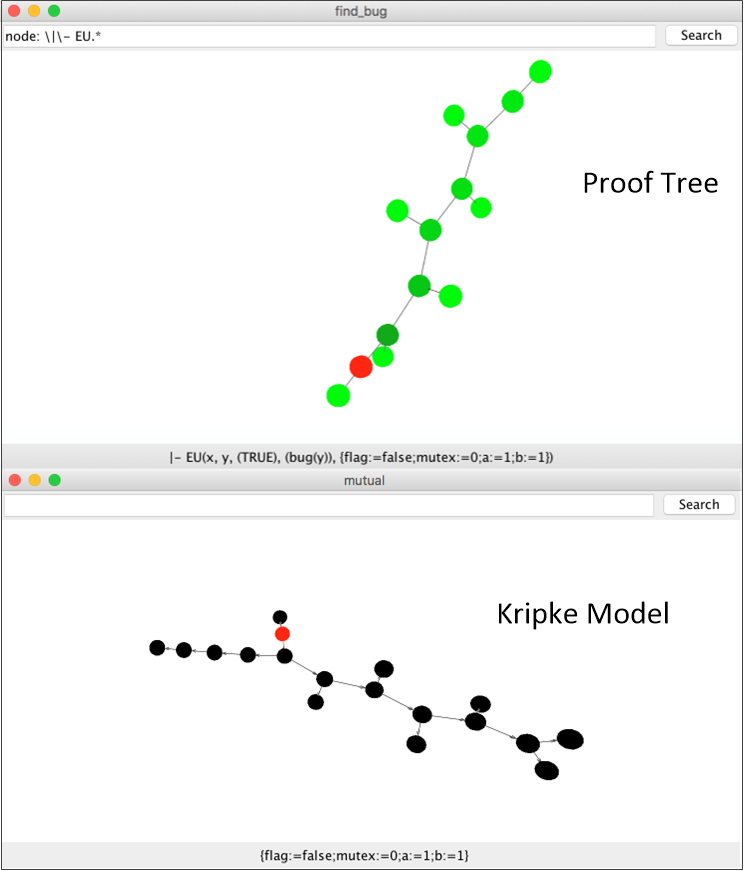
\includegraphics[width=10cm]{./illustrative_example2.png}
		\caption{进程互斥问题的验证中证明树和模型的可视化}
%		\caption{Visualization of the proof tree and the Kripke model in the illustrative example.}
		\label{fig:visualize:illustrative}
	\end{figure}
	
	通过对原程序进行修改\cite{Peterson81},可以使程序满足进程互斥性质,修改后的程序如图\ref{illustrative:mutual:solution}所示。修改后的程序可形式化描述为图\ref{fig:mutual:solution}所示的输入文件。在此输入文件中,变量$x$和变量$y$均为布尔变量,分别指代当前状态下进程$A$和进程$B$是否在运行,而$turn$则表示进程$A$和进程$B$轮流处在临界区内。
	\couic{Note that the violation of the mutual exclusion property can be avoided if the the algorithm of the two processes is modified \cite{Peterson81} as in Figure \ref{illustrative:mutual:solution}. The Kripke model built for this algorithm is depicted in Figure \ref{fig:mutual:solution}. Variable $x$ and $y$ are used to to indicate whether process A and B are running, respectively; $turn$ is the variable indicating it is whose turn to enter the critical section.}
	
	\begin{figure}[!h]
		\centering
		\small
		\begin{tabular}{p{5.8cm}p{4.8cm}}
			\begin{verbatim}
			/* Process A */
			1: x = true;
			2: turn = 1;
			3: while(y&&turn!=2); /*wait*/
			4: mutex ++;
			/*critical section*/
			5: mutex --;
			6: x = false;
			\end{verbatim}
			&
			\begin{verbatim}
			/* Process B */
			1: y = true;
			2: turn = 2;
			3: while(x&&turn!=1); /*wait*/
			4: mutex ++;
			/*critical section*/
			5: mutex --;
			6: y = false;
			\end{verbatim}
		\end{tabular}
		
		\caption{修改后的进程互斥程序。}
		\label{illustrative:mutual:solution}	
	\end{figure}
	
	\begin{figure}[h!]
		\centering
		\scriptsize
%		\begin{tabular}{|c|}
			
%		\begin{minipage}{10cm}
		\begin{boxedverbatim}
		Model mutual()
		{
		  Var {
		    x:Bool; y:Bool; mutex:(0 .. 2); turn:(1 .. 2); a:(1 .. 6); b:(1 .. 6);
		  }
		  Init {
		    x := false; y := false; mutex := 0; turn := 1; a := 1; b := 1;
		  }	
		  Transition {
		    a = 1 : {a := 2; x := true;};
		    a = 2 : {a := 3; turn := 1;};
		    a = 3 && (y = false || turn = 2): {a := 4;}; 
		    /*A has entered the critical section*/
		    a = 4 : {a := 5; mutex := mutex + 1;}; 
		    /*A has left the critical section*/
		    a = 5 : {a := 6; mutex := mutex - 1;}; 
		    a = 6 : {x := false;};
		    b = 1 : {b := 2; y := true;};
		    b = 2 : {b := 3; turn := 2;};
		    b = 3 && (x = false || turn = 1): {b := 4;}; 
		    /*B has entered the critical section*/
		    b = 4 : {b := 5; mutex := mutex + 1;}; 
		    /*B has left the critical section*/
		    b = 5 : {b := 6; mutex := mutex - 1;}; 
		    b = 6 : {y := false;};
		    /*If none of the conditions above are satisfied, 
		    then the current state goes to itself.*/
		    (a != 3 && (y = true && turn = 1)) || (b != 3 && (x = true && turn = 2)) : {};
		  }
		  Atomic {
		    bug(s) := s(mutex = 2);
		  }
		  Spec {
		    find_bug := EU(x, y, TRUE, bug(y), ini);
		  }
		}
		
		\end{boxedverbatim}
%	\end{minipage}
%	\end{tabular}
		\caption{输入文件“mutual\_solution.model”}
		\label{fig:mutual:solution}
	\end{figure}
	
	%	The verification result of this model would be as follows.
%	When applying this solution, the mutual exclusion exclusion property will not be violated, which is indicated by the following result.
	如下所示,修改后的程序满足进程互斥性质。
	\begin{center}
		\small
		\begin{verbatim}
             verifying on the model mutual...
             find_bug: EU(x, y, TRUE, bug(y), ini)
             find_bug is false.
		\end{verbatim}
	\end{center}
\end{example}

\subsection{案例二:小型飞机场运输系统}
在本小节中,我们介绍对于一个工程问题的形式化验证:由美国国家航空与航天局(National Aeronautics and Space Administration,简称NASA)为主导提出的小型飞机场运输系统(Small Aircraft Transportation System,简称SATS)\cite{MunozDC04,nasasats04}。在\sctlprov{}中,我们对SATS系统进行形式化描述,并验证该系统的安全性。
\couic{As an application to an engineering problem, we present
a concept of operations for the {\em Small Aircraft Transportation System} 
(\textsf{SATS}) 
\cite{MunozDC04,nasasats04}
in \sctl{}\footnote{\url{https://github.com/terminatorlxj/SATS-model}}.}



\begin{figure}
	\centering
	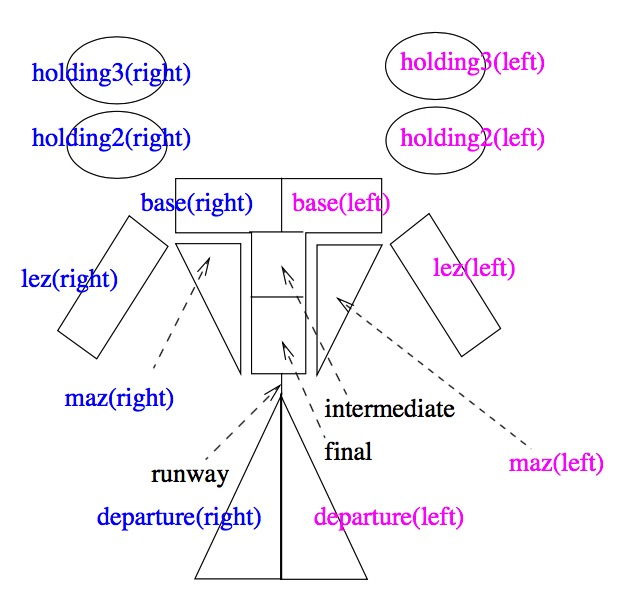
\includegraphics[width=9cm]{./sca.jpg}
	\caption{飞机场自我控制区域的划分(以飞行员视角区分左右)}
	%	\caption{SCA zones, where right and left are relative to the pilot facing the runway, i.e., opposite from the reader point of view \cite{MunozDC04}.}
	\label{fig:example:sats:sca}
\end{figure}

在SATS系统中,整个飞机场区域被称为自我控制区(Self Control Area,简称SCA)。如图\ref{fig:example:sats:sca}所示,该模型将SCA被分为15个子区域:
\begin{itemize}
	\item \textbf{holding3(right/left)}:等待航线,高度3000英尺(右/左);
	\item \textbf{holding2(right/left)}:等待航线,高度2000英尺(右/左);
	\item \textbf{lez(right/left)}:水平降落航线(右/左);
	\item \textbf{base(right/left)}:基地航线(右/左);
	\item \textbf{intermediate}:中间航线;
	\item \textbf{final}:最终航线;
	\item \textbf{runway}:机场跑道;
	\item \textbf{maz(right/left)}:重新降落航线(右/左);
	\item \textbf{departure(right/left)}:起飞航线(右/左)。
\end{itemize}
在任意时刻,SCA的每个子区域内都有若干架飞机,每个子区域内的飞机遵循先进先出的顺序依次进出。在整个SCA中,飞机的进出子区域的方式有24种,分别如下:
\begin{itemize}
	\item 进入3000英尺高度等待航线(右/左);
	\item 进入水平降落航线(右/左);
	\item 从3000英尺等待航线进入2000英尺等待航线(右/左);
	\item 从2000英尺等待航线进入基地航线(右/左);
	\item 从水平降落航线进入基地航线(右/左);
	\item 从基地航线(右/左)进入中间航线;
	\item 从中间航线进入重新降落航线(右/左);
	\item 从中间航线进入最终航线;
	\item 准备降落,从最终航线进入机场跑道;
	\item 降落成功,飞机驶离机场跑道;
	\item 降落失败,从最终航线进入重新降落航线(右/左);
	\item 从重新降落航线进入高度最低,而且可以进入(当前等待航线中没有飞机)的等待航线;
	\item 进入机场跑道并准备起飞;
	\item 从机场跑道进入起飞航线;
	\item 从起飞航线(右/左)离开,最终离开SCA。
\end{itemize}
在任意时刻,飞机进出SCA的子区域的方式必须是安全的,即SATS系统必须满足8个性质:
\begin{itemize}
	\item SCA中不超过4架飞机同时准备降落:即等待航线,水平降落航线,重新降落航线,基地航线,中间航线,以及最终航线上飞机的总数不超过4;
	\item SCA中左右两侧的航线(等待航线,水平降落航线,以及重新降落航线)中,同侧的飞机数总和不超过2,同时SCA中不超过2架飞机准备从同侧重新降落航线重新降落;
	\item 进入SCA的航线(等待航线和水平进入航线)中,每个航线每侧的飞机数不超过2,同时基地航线的飞机数总和不超过3;
	\item 在每侧的水平进入航线中最多只有一架飞机,同时如果某侧水平进入航线中有飞机,则SCA的同侧其他航线(水平降落航线以及重新降落航线)中没有飞机;
	\item SCA中的飞机按照事先给定的顺序依次进入SCA;
	\item 最先进入SCA中飞机一定最先降落;
	\item 机场跑道上最多只有一架飞机;
	\item 起飞航线上的飞机彼此必须相隔足够远的距离。
\end{itemize}
在\sctlprov{}中,我们针对SCA建立一个Kripke模型:模型中的状态用15个状态变量来表示,分别代表SCA中15个子区域,每个状态变量都是列表类型,代表该子区域内的若干架飞机;模型中包含24条迁移规则,分别指代SCA中的所有飞机在每个子区域间的24种进出方式;要验证的性质是一个\ctlpm{}公式,即在每个状态上,SCA都满足安全性质。该模型的输入文件可在因特网\footnote{\url{https://github.com/terminatorlxj/SATS-model}}上下载。

\sctlprov{}验证该模型用时26秒左右,运行环境为:Linux操作系统,内存3.0GB,2.93GHz$\times$4 CPU。验证过程中共访问54221个状态(Dowek,Mu\~noz和Carre\~no提出了的对SATS系统的一个简化版的PVS建模\cite{MunozDC04}中,该模型中可访问的状态数为2811)。
经\sctlprov{}验证,该模型满足安全性性质。


\couic{The model is
non-deterministic, that is, for a given state, several transitions are
possible and all must be considered.  As there are no a
priori bounds on the number of aircraft in each zone, the number of
states in the model is potentially infinite. However, the number of
states that are reachable from the initial state is finite: 
an enumeration of the model shows that there are 54221 such states (and
around 3000 in the simplified model where departure operations are not
considered).

There are eight properties of the model that we want to 
verify with \sctl{}, for instance that 
the \textsf{SATS} concept does not allow more than four simultaneous 
landing operations and none of the 
15 zones contains too many aircraft (each zone is
assigned a maximum number of aircraft and the actual number of
aircraft is never higher than this number).
The safety property is thus conjunction of these eight properties. 

The verification problem is to check that this
property holds on every reachable state from the initial state (the
state where there are no aircraft on each zone of the self controlled
area), so the formula to be checked is $AG_x(\phi)(e)$ where $\phi$ is 
the conjunction of the eight properties and $e$ is the initial state.
}

值得注意的是,虽然这是一个典型的模型检测问题,但是传统的模型检测工具均无法验证该模型\cite{MunozDC04},理由如下:
\couic{This is a typical model checking problem, but this problem
is known to be cumbersome for traditional model checkers
\cite{MunozDC04} because:}
\begin{enumerate}
	\couic{\item Each state of the model is represented by a complex data
	structure. For instance, a number of state variables are
	represented by lists of aircraft with unbounded length.}
	\item 模型的状态由复杂的数据结构所表示:每个状态变量的值均为列表类型,而且列表的长度可能为无穷。
	\couic{\item The transition rules of the model are 
	complex algorithms. For instance, some transitions rules
	involve recursive operations on lists of aircraft.}
	\item 状态的迁移规则必须由复杂的算法所描述:在某些状态迁移的过程中需要对飞机列表进行递归操作。
	\couic{\item The
	properties to be verified in the model are also represented
	by complex algorithms. For instance, some of the properties
	are inductively defined over lists of aircraft.}
	\item 模型的性质必须由复杂的算法所描述:某些原子命题的定义需要对飞机列表进行递归操作。
\end{enumerate}
\sctlprov{}的输入语言表达能力强于绝大多数模型检测工具,并能完整的表示该模型,同时成功进行验证。

\couic{However, this example fits well in \sctl{} that provides a
more expressive input language than most traditional model
checkers. Indeed, \sctl{} provides both readable notations for the
definition of data structures such as records or lists with unbounded
length, and arbitrary algorithms for the definitions of transition
rules and of properties.  So we have been able to check in
\sctl{} that the safety property holds on the model, and the
verification was executed in less than 30 seconds on the same machine as which the benchmarks are evaluated.}

\subsection{随机生成的布尔程序的验证}\label{subsec:random}
本小节包含三个测试集:测试用例集一在首次提出\cite{Zhang14}时被用作对比限界模型检测工具\verds{}和符号模型检测工具\nusmv{}的性能;并紧接着被用作对比定理证明器\tool{iProver Modulo}与\verds{}的性能;在测试集一的基础上,我们通过增大模型中的状态变量的个数而得到测试集二与测试集三。每个测试集中均包含2880个测试用例,每个测试用例的Kripke模型都是随机生成的,每个模型中的状态变量绝大多数为布尔类型。大量的随机的测试用例对于\sctlprov{}与不同的工具来说都是相对公平的,而且通过对比不同工具的实验结果数据,我们可以清晰的得出有关各个工具在验证不同的模型以及不同的性质时的优势与劣势的结论。

以下分别介绍这三个测试集。

\couic{We consider three benchmarks in this part. 
The original description of benchmark \#1 \cite{Zhang14} is restated here.
Based on benchmark \#1, we extend the number of variables to tens, hundreds, and even thousands in benchmark \#2 and benchmark \#3.
The randomness of the test cases in three benchmarks makes it rather fair for different \CTL{} model checking approaches, and helps us recognize the strengths and weaknesses of each tool. }

\subsubsection{测试集一}
Benchmark \#1 chosen in this subsection is originally introduced by Zhang \cite{Zhang14} in the evaluation of model checkers \verds{} and \nusmv{}. Later, Ji \cite{Ji15} also uses this benchmark in the evaluation of the theorem prover \tool{iProver Modulo} and the model checker \verds{}. This benchmark consists of 2880 randomly generated test cases where two types of random Boolean programs are considered---Concurrent Processes and Concurrent Sequential Processes. 
In programs with Concurrent Processes,
the parameters of the first set of random Boolean programs are as
follows.

测试集一中包含两类测试用例:并发进程(Concurrent Processes,简称CP)和并发顺序进程(Concurrent Sequential Processes,简称CSP)。
\paragraph{并发进程}
在描述并发进程需要用到以下4个变量:

\begin{center}
	\begin{tabular}{|l|}
		\hline
		$a$: 进程个数 \\
		$b$: 所有进程的共享变量和局部变量的个数 \\
		$c$: 进程间共享变量的个数 \\
		$d$: 每个进程的局部变量的个数 \\
		\hline
	\end{tabular}
\end{center}
进程间的共享变量的初始值均为$\{0,1\}$中的随机值,而每个进程的局部变量的初始值均为$0$。每个进程的共享变量和局部变量的每次赋值均为随机选择的某个变量的值的逻辑非。我们令进程个数为3,即$a=3$;令$b$在$\{12,24,36\}$中取值;同时令$c=b/2$,以及$d=c/a$。对于每个$b$的取值有20个Kripke模型,然后在每个Kripke模型分别验证24个\CTL{}性质。因此,此测试集中共有$3\times20\times24=1440$个并发进程测试用例。

\couic{The shared variables are initially set to a random value in $\{0,1\}$,
and the local variables are initially set to $0$. For each process,
the shared variables and the local variables are assigned the negation
of a variable randomly chosen from these variables. We test different
sizes of the programs with 3 processes ($a=3$), and let $b$ vary over
the set of values $\{12,24,36\}$, then set $c=b/2, d=c/a$. Each of the
24 properties is tested on 20 test cases for each value of $b$.}

\paragraph{并发顺序进程} 
在并发顺序进程测试用例中,除了以上定义的$a,b,c,d$变量之外,描述该类型测试用例还需用到以2个变量:

\couic{In programs with Concurrent Sequential Processes,
in addition to $a,b,c,d$ specified above, the parameters of the second set of random Boolean programs are as
follows.}
\begin{center}
	\begin{tabular}{|l|}
		\hline
		$t$: 每个进程的迁移的个数 \\
		$p$: 在每个迁移过程中同时进行的赋值的个数\\
		\hline
	\end{tabular}
\end{center}
For each concurrent sequential process, besides the $b$ Boolean
variables, there is a local variable representing program locations,
with $c$ possible values. The shared variables are initially set to a
random value in $\{0,1\}$, and the local variables are initially set
to $0$. For each transition of a process, $p$ pairs of shared
variables and local variables are randomly chosen among the shared
variables and the local variables, such that the first element of such
a pair is assigned the negation of the second element of the
pair. Transitions are numbered from $0$ to $t-1$, and are executed
consecutively, and when the end of the sequence of the transitions is
reached, it loops back to the execution of the transition numbered
$0$. For this type of programs, we test different sizes of the
programs with $2$ processes ($a=2$), and let $b$ vary in the set of
values $\{12,16,20\}$, and then set $c=b/2, d=c/a, t=c$, and
$p=4$. Similarly, each property is tested on $20$ test cases for each
value of $b$.


Twenty-four properties are to be checked in this benchmark: properties $P_{01}$ to $P_{12}$ are depicted in Figure~\ref{fig:properties}, and $P_{13}$ to $P_{24}$ are simply the variations of
$P_{01}$ to $P_{12}$ by replacing $\wedge$ and $\bigvee$ by $\vee$ and
$\bigwedge$, respectively.

\begin{figure}[!h]
	\centering
	{
		\begin{tabular}{|l|l|}
			\hline
			$P_{01}$& $AG(\bigvee^c_{i=1}v_i)$ \\
			\hline
			$P_{02}$& $AF(\bigvee^c_{i=1}v_i)$ \\
			\hline
			$P_{03}$& $AG(v_1 \A AF(v_2\wedge \bigvee^c_{i=3}v_i))$
			\\
			\hline
			$P_{04}$& $AG(v_1 \A EF(v_2\wedge \bigvee^c_{i=3}v_i))$
			\\
			\hline
			$P_{05}$& $EG(v_1 \A AF(v_2\wedge \bigvee^c_{i=3}v_i))$
			\\
			\hline
			$P_{06}$& $EG(v_1 \A EF(v_2\wedge \bigvee^c_{i=3}v_i))$
			\\
			\hline
			$P_{07}$& $AU(v_1, AU(v_2, \bigvee^c_{i=3}v_i))$\\
			\hline
			$P_{08}$ & $AU(v_1, EU(v_2, \bigvee^c_{i=3}v_i))$\\
			\hline
			$P_{09}$& $AU(v_1, AR(v_2, \bigvee^c_{i=3}v_i))$\\
			\hline
			$P_{10}$& $AU(v_1, ER(v_2, \bigvee^c_{i=3}v_i))$\\
			\hline
			$P_{11}$& $AR(AX v_1, AX AU(v_2, \bigvee^c_{i=3}v_i))$\\
			\hline
			$P_{12}$& $AR(EX v_1, EX EU(v_2, \bigvee^c_{i=3}v_i))$\\
			\hline
		\end{tabular}
	}
	\caption{测试集一、二、三中需要验证的性质$P_{01}, P_{02}, \ldots, P_{12}$}
	\label{fig:properties}
\end{figure}

\subsubsection{测试集二、三}
In benchmark {\#}2, we increase the number of state variables in benchmark \#1 to $48$, $60$, or $72$ for Concurrent Processes, and $24$,
$28$, or $32$ for Concurrent Sequential Processes. The 2880 test cases are also randomly generated.
The properties to be checked are the same as in benchmark \#1.

In benchmark {\#}3, we increase the number of state variables in benchmark \#1 to $252$, $504$
and $1008$ for both Concurrent Processes and Concurrent Sequential Processes, and check the same properties as benchmark \#1 and \#2.

\subsubsection{实验数据}
The experimental results are shown below, and the detailed data is in \ref{app:detail:data}.

\paragraph{Experimental data for benchmark \#1.}
For 2880 test cases in this benchmark, \tool{iProver Modulo} can solve 1816 (63.1\%) cases, \verds{} can solve 2230 (77.4\%) cases, \sctl{} can solve 2862 (99.4\%) cases, and both \nusmv{} and \nuxmv{} can solve all (100\%) test cases. The numbers of test cases where \sctl{} runs faster are 2823 (98.2\%) comparing with \tool{iProver Modulo}, 2858 (99.2\%) comparing with \verds{}, 2741 (95.2\%) comparing with \nusmv{}, and 2763 (95.9\%) comparing with \nuxmv{}. According to Figure~\ref{fig:average_time} and Figure~\ref{fig:average_memory}, \sctl{} uses less time and space than the other four tools.
\paragraph{Experimental data for benchmark \#2.}
For 2880 test cases in this benchmark, \tool{iProver Modulo} can solve 1602 (55.6\%) cases, \verds{} can solve 1874 (65.1\%) cases, \nusmv{} can solve 728 (25.3\%) cases, \nuxmv{} can solve 736 (25.6\%) cases, and \sctl{} can solve 2597 (90.2\%) cases. The numbers of test cases where \sctl{} runs faster are 2597 (90.2\%) comparing with \tool{iProver Modulo}, 2594 (90.1\%) comparing with \verds{}, and 2588 (89.9\%) comparing both with \nusmv{} and \nuxmv{}. According to Figure~\ref{fig:average_time:extended} and Figure~\ref{fig:average_memory:extended}, \sctl{} uses less time and space than the other four tools.
\paragraph{Experimental data for benchmark \#3.}
For 2880 test cases in this benchmark, \tool{iProver Modulo} can solve 1146 (39.8\%) cases, \verds{} can solve 352 (12.2\%) cases, \sctl{} can solve 1844 (64.0\%) cases, while neither \nusmv{} nor \nuxmv{} can solve any case.


\begin{figure}[h!]\centering
	%		\begin{subfigure}\centering
	\begin{tabular}{c}
		\scriptsize
		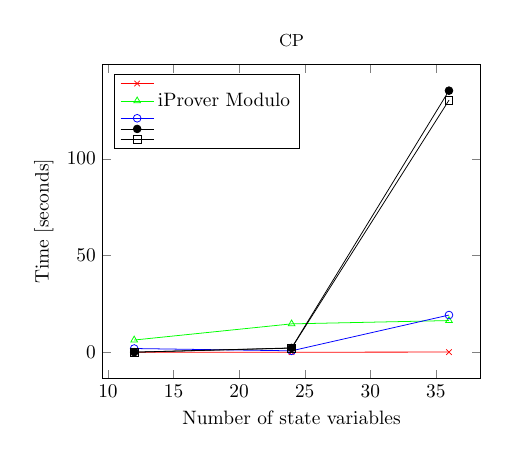
\begin{tikzpicture}[scale=0.7]
		\begin{axis}[title={\small{CP}},legend pos=north west, 
		% small,
		xlabel = {\normalsize Number of state variables},
		ylabel = {\normalsize Time [seconds]}
		]
		\addplot [color=red, mark=x] coordinates
		{
			(12,0.011)
			(24,0.010)
			(36,0.057)     
		};
		\addplot [color=green, mark=triangle] coordinates
		{
			(12,6.293)
			(24,14.648)
			(36,16.351)
		};
		\addplot [color=blue, mark=o] coordinates
		{
			(12,1.904)
			(24,0.714)
			(36,19.200)
		};
		\addplot [color=black,mark=*] coordinates
		{
			(12,0.014)
			(24,2.202)
			(36,135.202)
		};
		\addplot [color=black,mark=square] coordinates
		{
			(12,0.018)
			(24,2.100)
			(36,130.268)
		};
		{\legend{\sctl{},\tool{iProver Modulo}, \verds{}, \nusmv{}, \nuxmv{}}}
		\end{axis}
		\end{tikzpicture}
		
	\end{tabular}
	%		\end{subfigure}
	%		\begin{subfigure}
	%			\centering
	\begin{tabular}{c}
		\scriptsize
		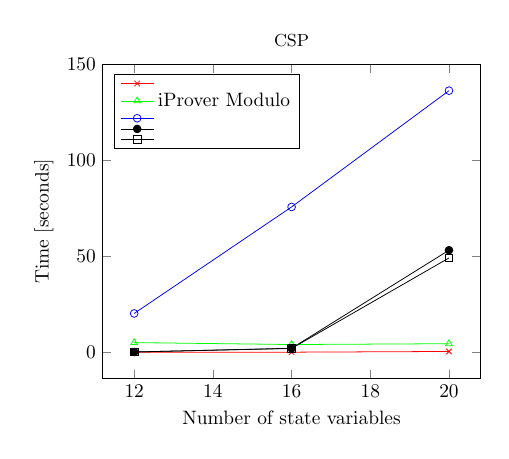
\begin{tikzpicture}[scale=0.7]
		\begin{axis}[title={\small{CSP}},legend pos=north west, 
		%small,
		xlabel = {\normalsize Number of state variables},
		ylabel = {\normalsize Time [seconds]}
		]
		\addplot [color=red, mark=x] coordinates
		{
			(12,0.006)
			(16,0.007)
			(20,0.374)      
		};
		\addplot [color=green, mark=triangle] coordinates
		{
			(12,4.995)
			(16,3.997)
			(20,4.424)
		};
		\addplot [color=blue, mark=o] coordinates
		{
			(12,20.203)
			(16,75.741)
			(20,136.387)
		};
		\addplot [color=black,mark=*] coordinates
		{
			(12,0.105)
			(16,2.036)
			(20,53.195)
		};
		\addplot [color=black,mark=square] coordinates
		{
			(12,0.107)
			(16,1.957)
			(20,49.144)
		};
		{\legend{\sctl{},\tool{iProver Modulo}, \verds{}, \nusmv{}, \nuxmv{}}}
		\end{axis}
		\end{tikzpicture}
	\end{tabular}
	%		\end{subfigure}
	
	\caption{Average verification time in benchmark {\#}1.}
	\label{fig:average_time}
	\end{figure}
	
	\begin{figure}[h!]\centering
%	\begin{subfigure}\centering
		\begin{tabular}{c}
			\scriptsize
			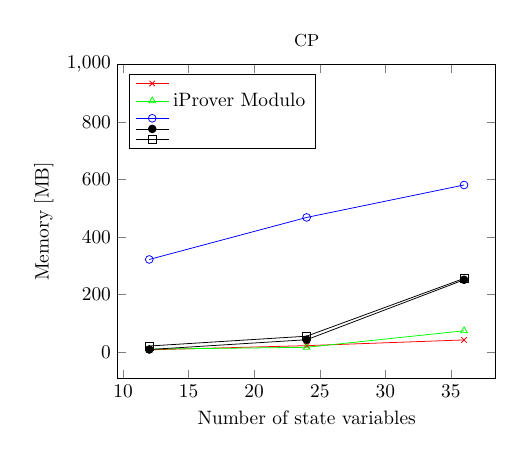
\begin{tikzpicture}[scale=0.7]
			\begin{axis}[title={\small{CP}},legend pos=north west, 
			%small, 
			ymax=1000,
			xlabel = {\normalsize Number of state variables},
			ylabel = {\normalsize Memory [MB]}
			]
			\addplot [color=red, mark=x] coordinates
			{
				(12,7.845)
				(24,22.328)
				(36,42.184)     
			};
			\addplot [color=green, mark=triangle] coordinates
			{
				(12,10.111)
				(24,16.547)
				(36,73.946)
			};
			\addplot [color=blue, mark=o] coordinates
			{
				(12,322.020)
				(24,468.169)
				(36,581.011)
			};
			\addplot [color=black,mark=*] coordinates
			{
				(12,8.818)
				(24,42.924)
				(36,251.364)
			};
			\addplot [color=black,mark=square] coordinates
			{
				(12,21.013)
				(24,55.179)
				(36,256.058)
			};
			\legend{\sctl{},\tool{iProver Modulo}, \verds{}, \nusmv{}, \nuxmv{}}
			\end{axis}
			\end{tikzpicture}
			
		\end{tabular}
%	\end{subfigure}
%	\begin{subfigure}
%		\centering
		\begin{tabular}{c}
			\scriptsize
			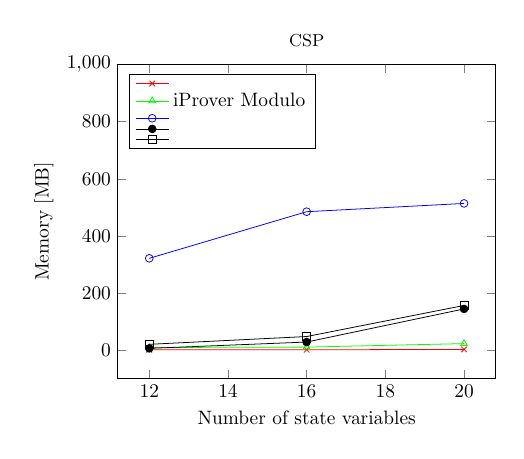
\begin{tikzpicture}[scale=0.7]
			\begin{axis}[title={\small{CSP}},legend pos=north west, 
			%small, 
			ymax=1000,
			xlabel = {\normalsize Number of state variables},
			ylabel = {\normalsize Memory [MB]}
			]
			\addplot [color=red, mark=x] coordinates
			{
				(12,1.984)
				(16,2.039)
				(20,3.383)      
			};
			\addplot [color=green, mark=triangle] coordinates
			{
				(12,10.070)
				(16,11.449)
				(20,23.660)
			};
			\addplot [color=blue, mark=o] coordinates
			{
				(12,322.023)
				(16,485.081)
				(20,514.027)
			};
			\addplot [color=black,mark=*] coordinates
			{
				(12,7.051)
				(16,29.151)
				(20,144.974)
			};
			\addplot [color=black,mark=square] coordinates
			{
				(12,21.168)
				(16,48.423)
				(20,157.113)
			};
			{\legend{\sctl{},\tool{iProver Modulo}, \verds{}, \nusmv{}, \nuxmv{}}}
			\end{axis}
			\end{tikzpicture}
		\end{tabular}
%	\end{subfigure}
	
	\caption{Average memory usage in benchmark {\#}1.}
	\label{fig:average_memory}
\end{figure}


\begin{figure}[h!]\centering
%	\begin{subfigure}\centering
		\begin{tabular}{c}			
			\scriptsize
			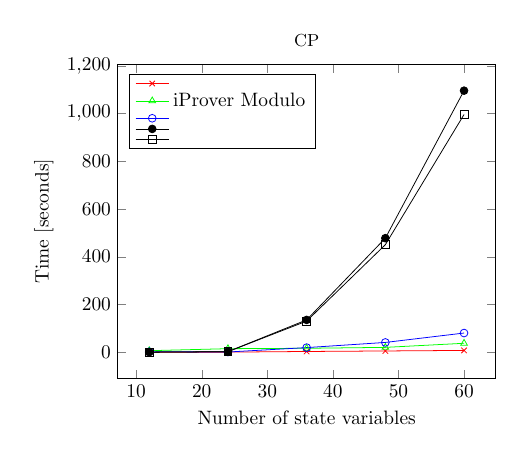
\begin{tikzpicture}[scale=0.7]
			\begin{axis}[title={\small{CP}},legend pos=north west, 
			%small,
			xlabel = {\normalsize Number of state variables},
			ylabel = {\normalsize Time [seconds]}
			]
			\addplot [color=red, mark=x] coordinates
			{
				(12,0.011)
				(24,0.280)
				(36,2.929)  
				(48,5.100)
				(60,7.357)   
			};
			\addplot [color=green, mark=triangle] coordinates
			{
				(12,6.293)
				(24,14.648)
				(36,16.351)
				(48,20.130)
				(60,37.303) 
			};
			\addplot [color=blue, mark=o] coordinates
			{
				(12,1.904)
				(24,0.714)
				(36,19.200)
				(48,40.825)
				(60,80.201)
			};
			\addplot [color=black,mark=*] coordinates
			{
				(12,0.014)
				(24,2.202)
				(36,135.202)
				(48,477.578)
				(60,1095.582)
			};
			\addplot [color=black,mark=square] coordinates
			{
				(12,0.018)
				(24,2.100)
				(36,130.268)
				(48,450.324)
				(60,995.689)
			};
			\legend{\sctl{}, \tool{iProver Modulo}, \verds{}, \nusmv{}, \nuxmv{}}
			\end{axis}
			\end{tikzpicture}
			
		\end{tabular}
%	\end{subfigure}
%	\begin{subfigure}
%		\centering
		\begin{tabular}{c}
			\scriptsize
			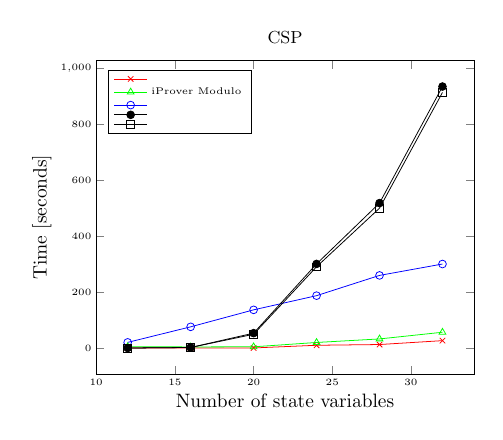
\begin{tikzpicture}[scale=0.7]
			\begin{axis}[title={\small{CSP}},legend pos=north west, 
			%small,
			xlabel = {\normalsize Number of state variables},
			ylabel = {\normalsize Time [seconds]}
			]
			\addplot [color=red, mark=x] coordinates
			{
				(12,0.006)
				(16,0.007)
				(20,0.374) 
				(24,9.903)
				(28,12.548)
				(32,26.417)     
			};
			\addplot [color=green, mark=triangle] coordinates
			{
				(12,4.995)
				(16,3.997)
				(20,4.424)
				(24,19.903)
				(28,32.548)
				(32,56.417)   
			};
			\addplot [color=blue, mark=o] coordinates
			{
				(12,20.203)
				(16,75.741)
				(20,136.387)
				(24,187.043)
				(28,259.342)
				(32,300.031)
			};
			\addplot [color=black,mark=*] coordinates
			{
				(12,0.105)
				(16,2.036)
				(20,53.195)
				(24,300.406)
				(28,517.544)
				(32,933.722)
				
			};
			\addplot [color=black,mark=square] coordinates
			{
				(12,0.107)
				(16,1.957)
				(20,49.144)
				(24,290.205)
				(28,499.454)
				(32,912.527)
			};
			\tiny{\legend{\sctl{}, \tool{iProver Modulo}, \verds{}, \nusmv{}, \nuxmv{}}}
			\end{axis}
			\end{tikzpicture}
		\end{tabular}
%	\end{subfigure}
	
	\caption{Average verification time in benchmark \#1 and {\#}2.}
	\label{fig:average_time:extended}
	\end{figure}
	
	\begin{figure}[h!]\centering
		\scriptsize
%	\begin{subfigure}\centering
		\begin{tabular}{c}
			
			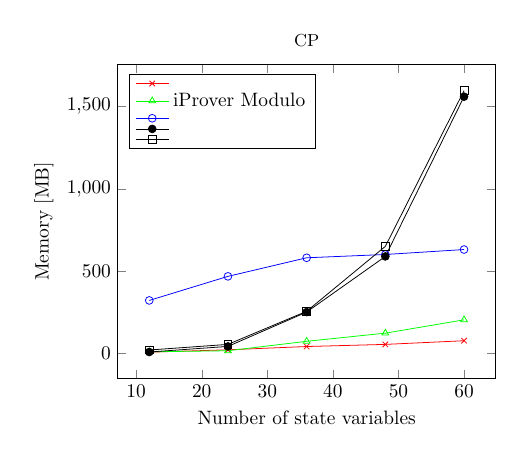
\begin{tikzpicture}[scale=0.7]
			\begin{axis}[title={\small{CP}},legend pos=north west, 
			%small,
			xlabel = {\normalsize Number of state variables},
			ylabel = {\normalsize Memory [MB]}
			]
			\addplot [color=red, mark=x] coordinates
			{
				(12,7.845)
				(24,22.328)
				(36,42.184)  
				(48,55.100)
				(60,77.357)   
			};
			\addplot [color=green, mark=triangle] coordinates
			{
				(12,10.111)
				(24,16.547)
				(36,73.946)
				(48,123.342)
				(60,204.298)
			};
			\addplot [color=blue, mark=o] coordinates
			{
				(12,322.020)
				(24,468.169)
				(36,581.011)
				(48,601.023)
				(60,631.034)
			};
			\addplot [color=black,mark=*] coordinates
			{
				(12,8.818)
				(24,42.924)
				(36,251.364)
				(48,589.205)
				(60,1559.283)
			};
			\addplot [color=black,mark=square] coordinates
			{
				(12,21.013)
				(24,55.179)
				(36,256.058)
				(48,650.324)
				(60,1595.689)
			};
			\legend{\sctl{}, \tool{iProver Modulo}, \verds{}, \nusmv{}, \nuxmv{}}
			\end{axis}
			\end{tikzpicture}
			
		\end{tabular}
%	\end{subfigure}
%	\begin{subfigure}
%		\centering
		\begin{tabular}{c}
			\scriptsize
			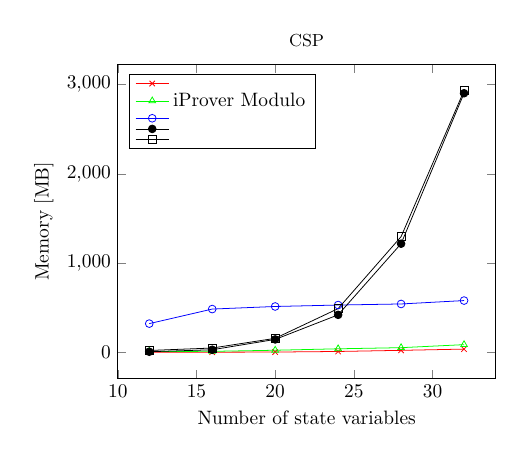
\begin{tikzpicture}[scale=0.7]
			\begin{axis}[title={\small{CSP}},legend pos=north west, 
			%small,
			xlabel = {\normalsize Number of state variables},
			ylabel = {\normalsize Memory [MB]}
			]
			\addplot [color=red, mark=x] coordinates
			{
				(12,1.984)
				(16,2.039)
				(20,3.383) 
				(24,9.903)
				(28,22.548)
				(32,36.417)     
			};
			\addplot [color=green, mark=triangle] coordinates
			{
				(12,10.070)
				(16,11.449)
				(20,23.660)
				(24,39.903)
				(28,52.548)
				(32,86.417)
			};
			\addplot [color=blue, mark=o] coordinates
			{
				(12,322.023)
				(16,485.081)
				(20,514.027)
				(24,530.238)
				(28,542.231)
				(32,580.357)
			};
			\addplot [color=black,mark=*] coordinates
			{
				(12,7.051)
				(16,29.151)
				(20,144.974)
				(24,420.406)
				(28,1217.544)
				(32,2903.722)
				
			};
			\addplot [color=black,mark=square] coordinates
			{
				(12,21.168)
				(16,48.423)
				(20,157.113)
				(24,490.205)
				(28,1296.454)
				(32,2932.527)
			};
			{\legend{\sctl{}, \tool{iProver Modulo}, \verds{}, \nusmv{}, \nuxmv{}}}
			\end{axis}
			\end{tikzpicture}
		\end{tabular}
%	\end{subfigure}
	
	\caption{Average memory usage in benchmark \#1 and {\#}2.}
	\label{fig:average_memory:extended}
\end{figure}



\subsubsection{连续 vs. 递归}
To show the importance of using continuation-passing style,
we have implemented a recursive version of our tool and compared the time
efficiency. In benchmark {\#}1, {\#}2, and {\#}3, \sctl{} solves about 10\% more test cases than \sctlprovr{}, and it outperforms \sctlprovr{} in almost
all solvable cases (Table~\ref{tabl:cont_vs_rec}). \sctlprovr{} is more sensitive to the number of variables than \sctl{} (Figure \ref{fig:average_time:recursive:vs:continuation}).

{
	\begin{table}
		\setlength{\tabcolsep}{1pt}
		\begin{center}
			\begin{tabular}{| l | r | r | r |}
				
				\hline
				\textbf{Bench} & \sctl{} solvable & \sctlprovr{} solvable & t(\sctlprov) $<$ t(\sctlprovr{})  \\
				\hline
				%\code{CP} & 1430(99.3\%) & 1354(94.0\%) \\
				%\hline
				%\code{CSP} & 1432(99.4\%) & 1328(92.2\%) \\
				%\hline
				\textbf{\#1} & 2862(99.4\%) & 2682(93.1\%) & 2598(90.2\%)\\
				\hline
				\textbf{\#2} & 2597(90.2\%) & 2306(80.1\%) & 2406(83.5\%)\\
				\hline
				\textbf{\#3} & 1849(64.2\%) & 1520(52.8\%) & 1735(60.2\%)\\
				\hline
			\end{tabular}
		\end{center}
		\caption{\sctl{} vs. \sctlprovr{}}
		\label{tabl:cont_vs_rec}
	\end{table}
}

\begin{figure}[h!]\centering
%	\begin{subfigure}\centering
		\begin{tabular}{c}
			\scriptsize
			\begin{tikzpicture}[scale=0.7]
			\begin{axis}[title={\small{CP}},legend pos=north west, 
			%small,
			xlabel = {\normalsize Number of state variables},
			ylabel = {\normalsize Time [seconds]}
			]
			\addplot [color=red, mark=x] coordinates
			{
				(12,0.011)
				(24,0.280)
				(36,2.929)  
				(48,5.100)
				(60,7.357)
				(72,19.566)   
			};
			\addplot [color=black,mark=*] coordinates
			{
				(12,0.032)
				(24,2.238)
				(36,6.717)
				(48,17.578)
				(60,55.582)
				(72,101.265)
			};
			\legend{\sctlprov, \sctlprovr{}}
			\end{axis}
			\end{tikzpicture}
			
		\end{tabular}
%	\end{subfigure}
%	\begin{subfigure}
		\centering
		\begin{tabular}{c}
			\scriptsize
			\begin{tikzpicture}[scale=0.7]
			\begin{axis}[title={\small{CSP}},legend pos=north west, 
			%small,
			xlabel = {\normalsize Number of state variables},
			ylabel = {\normalsize Time [seconds]}
			]
			\addplot [color=red, mark=x] coordinates
			{
				(12,0.006)
				(16,0.007)
				(20,0.374) 
				(24,9.903)
				(28,12.548)
				(32,26.417)
				(52,91.134)
				(72,180.098)     
			};
			
			\addplot [color=black,mark=*] coordinates
			{
				(12,0.035)
				(16,1.238)
				(20,10.717)
				(24,30.406)
				(28,57.544)
				(32,83.722)
				(52,234.546)
				(72,504.256) 
				
			};
			{\legend{\sctlprov,\sctlprovr{}}}
			\end{axis}
			\end{tikzpicture}
		\end{tabular}
%	\end{subfigure}
	
	\caption{Average verification time in \sctl{} vs. \sctlprovr.}
	\label{fig:average_time:recursive:vs:continuation}
\end{figure}


%\begin{remark}
	In the comparison of average verification time of \sctl{} and \sctlprovr, we extend the number of variables in Concurrent Sequential Processes to 52 and 72, on the basis of benchmark \#2.
%\end{remark}

\subsection{带有公平性性质的程序的验证}\label{subsec:fair}
%	We evaluate two benchmarks in this part: benchmark \#4 models the alternating bit protocol, and
In this part, we evaluate benchmark \#4, which models mutual exclusion
algorithms and ring
algorithms\footnote{\url{http://lcs.ios.ac.cn/~zwh/verds/verds_code/bp12.rar}}.
Then, we compare the evaluation results of \sctl{}, \verds{},
\nusmv{}, and \nuxmv{}, and we do not consider \tool{iProver Modulo}
because \tool{iProver Modulo} cannot handle \CTL{} properties with
fairness constraints \cite{Ji15}.


\paragraph{互斥算法和环算法 Mutual exclusion and ring algorithms.}

This benchmark consists of two sets of concurrent programs: the mutual
exclusion algorithms and the ring algorithms. Both kinds of algorithms
consist of a set of concurrent processes running in parallel. 


In the mutual exclusion algorithms, the scheduling of processes is simple: for all $i$ between $0$ and $n-2$, process $i+1$ performs a transition after process $i$, and process $0$ performs a transition after process $n-1$.
Each formula in the algorithms needs to be
verified under the fairness constraint that each process does not
starve, i.e., no process waits infinitely long.

Each process in the mutual exclusion algorithms has three internal
states: \textsf{noncritical}, \textsf{trying}, and
\textsf{critical}. The number of processes vary from $6$ to $51$. There
are five properties specified by \CTL{} formulae are to be verified in
mutual exclusion algorithms, as in
Table~\ref{tabl:mutual:ring:properties}. In these formulae, $non_i$
($try_i$, $cri_i$) indicates that process $p_i$ has internal state
\textsf{noncritical} (\textsf{trying}, \textsf{critical}).
Note that because of the scheduling algorithm, 
processes $0$ and $1$ are not symmetric, as exemplified by the 
difference in performance between the properties $P_4$ and $P_5$.

Each process in the ring algorithms consists of $5$ Boolean internal variables indicating the internal state, and a Boolean variable indicating the output. Each process receives a Boolean value as the input during its running time. For a ring algorithm with processes $p_0,p_1,...,p_n$, the internal state of $p_i$ depends on the output of process $p_{i-1}$, and the output of $p_{i-1}$ depends on its internal state, where $1\le i\le n$. The internal state of $p_0$ depends on the output of process $p_n$, and the output of $p_n$ depends on the internal state of its own. The number of processes vary from $3$ to $10$. There are four properties specified by \CTL{} formulae are to be verified in ring algorithms, as in Figure~\ref{tabl:mutual:ring:properties}. In these formulae, $out_i$ indicates that the output of process $p_i$ is Boolean value $true$.


%	The experimental results are shown in Table~\ref{tabl:solvable:mutual:ring}, \ref{tabl:compare:mutual:ring}, and \ref{tabl:data:mutual:ring}. 

The experimental results (Table~\ref{tabl:solvable:mutual:ring} and Table \ref{tabl:compare:mutual:ring}) show that \sctl{} solves more test cases than \verds, \nusmv{}, and \nuxmv{}. At the same time, \sctl{} is more time and space efficiency in more than 75 percent of the test cases than the other three tools.  

The detailed experimental data is shown in ~\ref{bench4:data:detail}.

\begin{table}
	%\setlength{\tabcolsep}{3pt}
	%\renewcommand{\arraystretch}{1.0}
	\begin{center}
		\begin{tabular}{| l | l |}
			\hline
			\textbf{Prop} & \textbf{Mutual Exclusion Algorithms}\\
			\hline
			{$P_1$} & $EF (cri_0 \wedge cri_1)$  \\
			\hline
			{$P_2$} &  $AG (try_0 \Rightarrow AF (cri_0))$\\
			\hline
			{$P_3$} &  $AG (try_1 \Rightarrow AF (cri_1))$\\
			
			\hline
			{$P_4$} &  $AG (cri_0 \Rightarrow A cri_0 U (\neg cri_0 \wedge A \neg cri_0 U cri_1))$  \\
			\hline
			{$P_5$} &  $AG (cri_1 \Rightarrow A cri_1 U (\neg cri_1 \wedge A \neg cri_1 U cri_0))$\\
			\hline
			%			\vspace{0.5cm}\\
			%		\end{tabular}
			%	\begin{tabular}{| l | l |}
			\hline
			\textbf{Prop} & \textbf{Ring Algorithms}\\
			\hline
			{$P_1$} & $AGAF out_0 \wedge AGAF \neg out_0$ \\
			\hline
			{$P_2$} &  $AGEF out_0 \wedge AGEF \neg out_0$ \\
			\hline
			{$P_3$} &  $EGAF out_0 \wedge EGAF \neg out_0$\\
			
			\hline
			{$P_4$} &  $EGEF out_0 \wedge EGEF \neg out_0$ \\
			\hline
		\end{tabular}
	\end{center}
	\figcaption{Properties to be verified in benchmark \#4.}
	\label{tabl:mutual:ring:properties}
\end{table}

\begin{table}
	%\setlength{\tabcolsep}{3pt}
	%\renewcommand{\arraystretch}{1.0}
	%	\begin{tabular}{c c}
	%		\begin{minipage}[b]{0.45\linewidth}
	\centering
	\setlength{\tabcolsep}{3pt}
	\begin{tabular}{| l | r | r | r | r |}
		\hline
		\textbf{Programs} & \verds{} & \nusmv{} & \nuxmv{} &  \sctl{} \\
		\hline
		\code{mutual exclusion} & 136 (59.1\%) & 50 (21.7\%) & 50 (21.7\%) & 191 (83.0\%)  \\
		\hline
		\code{ring} & 16 (50.0\%) & 21 (65.6\%) & 21 (65.6\%) & 20 (62.5\%) \\
		\hline
		Sum & 152(58.0\%) & 71(27.1\%) & 71(27.1\%) & 211 (80.5\%)\\
		\hline
	\end{tabular}	
	\caption{Solvable cases in \verds{}, \nusmv{}, \nuxmv{}, and \sctl{}.}
	\label{tabl:solvable:mutual:ring}
	\vspace{0.5cm}
	%\end{table}
	%\begin{table}
	%\scriptsize
	%			\centering
	%			\setlength{\tabcolsep}{3pt}
	\begin{tabular}{| l | r | r | r |}
		\hline
		\textbf{Programs} & \verds{} & \nusmv{} & \nuxmv{}  \\
		\hline
		\code{mutual exclusion} & 187 (81.3\%) & 191 (83.0\%) & 191 (83.0\%)   \\
		\hline
		\code{ring} & 13 (40.6\%) & 20 (62.5\%) & 20 (62.5\%)  \\
		\hline
		Sum & 200(76.3\%) & 211(80.5\%) & 211(80.5\%) \\
		\hline
	\end{tabular}
	\caption{Cases where \sctl{} both runs faster and uses less memory.}
	\label{tabl:compare:mutual:ring}
	%		\end{minipage}
	%	\end{tabular}
\end{table}


\subsection{工业级测试用例的验证}	\label{subsc:vlts}
In this part, we evaluate benchmark \#5, also called the \textsf{VLTS} (Very Large Transition Systems) benchmark\footnote{\url{http://cadp.inria.fr/resources/vlts/}}, which was originally proposed as a part of the \CADP{}\footnote{\url{http://cadp.inria.fr/}} (Construction and Analysis of Distributed Processes) toolbox \cite{GaravelLMS13}.
As a formal verification toolbox, \CADP{} focuses on action-based models, for instance, \textsf{LTS}s and Markov Chains.
As pointed out by the authors of \textsf{CADP}: \textit{this benchmark has been obtained from the modeling of various communication protocols and concurrent systems, many of which corresponds to real life and industrial systems}. 


There are 40 test cases in benchmark \#5, where deadlocks and livelocks are to be detected for each test case.
All test cases in benchmark \#5 are encoded as \textsf{BCG} (Binary-Coded Graphs) format, which is a binary format designed for encoding large state spaces \cite{GaravelLMS13}. 
When verifying test cases in this benchmark in \sctlprov{}, each \textsf{BCG} file was parsed into a Kripke model, and perform the proving procedure on the Kripke model. We compare the experimental results of detecting deadlocks and livelocks both in \sctlprov{} and \CADP{}. 

The experimental result is depicted in Table \ref{tabl:vlts}:
when detecting deadlocks, \sctlprov{} uses less time than \CADP{} in 31 (77.5\%) test cases, and uses less memory than \CADP{} in 35 (87.5\%) test cases;
when detecting livelocks, \sctlprov{} uses less time than \CADP{} in 22 (55\%) test cases, and uses less memory than \CADP{} in 27 (67.5\%) test cases.

For brevity's sake, more details about the experiment on benchmark \#5 are explained in \ref{appendix:data:benchmark5}.

\begin{figure}[h]
	
	\centering
	\begin{tabular}{ | l | c | c | }
		\hline
		\textbf{Cases} & t(\sctlprov) $<$ t(\CADP{}) & m(\sctlprov) $<$ m(\CADP{})\\\hline
		\code{deadlock} & 31 (77.5\%) & 35 (87.5\%)\\\hline
		\code{livelock} & 22 (55\%) & 27 (67.5\%)\\\hline
		%\hline
	\end{tabular}
	
	\tabcaption{Test cases where \sctlprov{} uses less time and less memory, respectively.}
	\label{tabl:vlts}
\end{figure}



\subsection{关于实验结果的讨论}
In the evaluation of benchmark \#1 to benchmark \#4 in this paper, the performances of \nusmv{}, \nuxmv{}, \verds{}, \tool{iProver Modulo}, and \sctl{} in the comparisons are affected by two factors: the number of state variables, and the type of the property to be checked. The performances of \nusmv{} and \nuxmv{} are mainly affected by the number of state variables, while the performances of \tool{iProver Modulo}, \verds{}, and \sctl{} are mainly affected by the type of the property to be checked. When the number of state variables is rather small (such as test cases in benchmark \#1), \nusmv{} and \nuxmv{} solves more test cases than \tool{iProver Modulo}, \verds{} and \sctl{}, but when the number of state variables becomes larger (such as test cases in benchmark \#2 and \#3), they performs worse than the other three tools.  When checking properties where nearly all states must be searched (such as $AG$ properties), \nusmv{} and \nuxmv{} usually perform better than \tool{iProver Modulo}, \verds{} and \sctl{}. However, for most properties, \tool{iProver Modulo}, \verds{} and \sctl{} usually search much less states than \nusmv{} and \nuxmv{} to check them, and are more time and space efficiency. Thus, \tool{iProver Modulo}, \verds{} and \sctl{} scale up better than \nusmv{} and \nuxmv{} when checking these properties. Moreover, \sctl{} scales up better than both \tool{iProver Modulo} and \verds{}, and outperforms these two tools in most solvable cases.


In the evaluation of benchmark \#5, the performances of \sctl{} and \CADP{} are affected by both the size of the state space, and the properties to be verified. 
The verification processes in \sctl{} and \CADP{} tend to use less time and memory in test cases which have smaller state spaces.
For test cases where there exists a deadlock or livelock, the verification processes tend to use less time and memory than those where there are no deadlock or livelock.
Moreover, \sctl{} outperforms \CADP{} in more than half of the test cases.  

